\documentclass[11pt,a4paper,oneside]{book}
% shared preamble of the user manual and the code reference
\usepackage[a4paper,margin=2.3cm,top=2.4cm,bottom=2.6cm]{geometry}
\usepackage{fontspec}
\usepackage{unicode-math}
\setmainfont{Latin Modern Roman}
\setsansfont{Latin Modern Sans}
\setmonofont{DejaVu Sans Mono}[Scale=0.80]
\setmathfont{Latin Modern Math}
\usepackage{amsmath}
\usepackage{xcolor}
\usepackage{graphicx}
\usepackage{booktabs,longtable,tabularx,array}
\usepackage{enumitem}
\usepackage{listings}
\usepackage[most]{tcolorbox}
\usepackage{fancyhdr}
\usepackage{titlesec}
\usepackage{tikz}
\usetikzlibrary{arrows.meta,positioning,shapes.geometric,calc,3d}
\usepackage{microtype}
\usepackage{caption}
\usepackage[colorlinks=true,linkcolor=blue!50!black,urlcolor=blue!50!black,citecolor=blue!50!black]{hyperref}

\definecolor{codebg}{RGB}{248,248,246}
\definecolor{codeframe}{RGB}{210,210,205}
\definecolor{kw}{RGB}{0,70,150}
\definecolor{cm}{RGB}{110,110,110}
\definecolor{st}{RGB}{150,60,0}
\definecolor{accent}{RGB}{30,80,140}
\definecolor{notebg}{RGB}{236,243,250}
\definecolor{warnbg}{RGB}{252,243,230}

\lstdefinestyle{py}{
  language=Python, basicstyle=\ttfamily\small, columns=fullflexible, keepspaces=true,
  keywordstyle=\color{kw}\bfseries, commentstyle=\color{cm}\itshape, stringstyle=\color{st},
  numbers=left, numberstyle=\ttfamily\scriptsize\color{gray}, numbersep=6pt,
  backgroundcolor=\color{codebg}, frame=single, rulecolor=\color{codeframe},
  breaklines=true, breakatwhitespace=false, postbreak=\mbox{\textcolor{gray}{$\hookrightarrow$}\space},
  showstringspaces=false, tabsize=4, xleftmargin=2.2em, framexleftmargin=2.0em,
  upquote=true, aboveskip=6pt, belowskip=4pt,
  morekeywords={self,None,True,False,as,with,yield,lambda,nonlocal}
}
\lstdefinestyle{plain}{
  basicstyle=\ttfamily\small, columns=fullflexible, keepspaces=true, numbers=none,
  backgroundcolor=\color{codebg}, frame=single, rulecolor=\color{codeframe},
  breaklines=true, showstringspaces=false, upquote=true, aboveskip=6pt, belowskip=6pt,
  xleftmargin=0.3em, framexleftmargin=0.2em
}
\lstdefinestyle{pyex}{style=py, numbers=none, xleftmargin=0.3em, framexleftmargin=0.2em}
\lstset{style=plain}

\newtcolorbox{note}[1][Note]{colback=notebg,colframe=accent,boxrule=0.5pt,arc=2pt,
  left=6pt,right=6pt,top=4pt,bottom=4pt,fonttitle=\bfseries\small,title=#1}
\newtcolorbox{warn}[1][Caution]{colback=warnbg,colframe=orange!70!black,boxrule=0.5pt,arc=2pt,
  left=6pt,right=6pt,top=4pt,bottom=4pt,fonttitle=\bfseries\small,title=#1}

\newcommand{\code}[1]{\texttt{#1}}
\newcommand{\Rsun}{R_\odot}
\newcommand{\rsun}{\ensuremath{R_\odot}}
\newcommand{\vect}[1]{\mathbf{#1}}

% line-by-line commentary list
\newlist{lines}{description}{1}
\setlist[lines]{font=\ttfamily\small\color{accent},leftmargin=5.2em,labelwidth=4.8em,
  labelsep=0.4em,itemsep=1pt,parsep=1pt,topsep=3pt,align=right}

\titleformat{\chapter}[display]{\normalfont\bfseries\color{accent}}{\large\scshape Chapter \thechapter}{4pt}{\huge}
\titlespacing*{\chapter}{0pt}{-10pt}{18pt}
\titleformat{\section}{\normalfont\Large\bfseries\color{accent}}{\thesection}{0.7em}{}
\titleformat{\subsection}{\normalfont\large\bfseries}{\thesubsection}{0.7em}{}

\pagestyle{fancy}
\fancyhf{}
\fancyhead[L]{\small\itshape radiosynth v2.2}
\fancyhead[R]{\small\nouppercase{\leftmark}}
\fancyfoot[C]{\small\thepage}
\renewcommand{\headrulewidth}{0.4pt}
\setlength{\headheight}{14pt}

\setlength{\parindent}{0pt}
\setlength{\parskip}{5pt plus 1pt}


\usepackage{xr}
\externaldocument{radiosynth_user_manual}
\hypersetup{pdftitle={radiosynth Line-by-line Code Reference},
  pdfsubject={Line-by-line description of the radiosynth source code}}
\begin{document}
\frontmatter
\begin{titlepage}
\centering
\vspace*{3cm}
{\Huge\bfseries\color{accent} radiosynth\par}
\vspace{0.25cm}
{\huge\itshape From MHD to MHz\par}
\vspace{0.6cm}
{\LARGE Synthetic Radio Imaging of MHD Solar--Stellar\\[2pt] Coronal Model Output and Comparison with Observations\par}
\vspace{0.4cm}
{\large A standalone Python implementation of the BATS-R-US refractive radio ray-tracing tool,\\ with thermal free--free, gyroresonance and gyrosynchrotron emission and circular polarisation,\\ for BATS-R-US, PLUTO and other MHD codes --- the Sun and other stars\par}
\vspace{1.5cm}
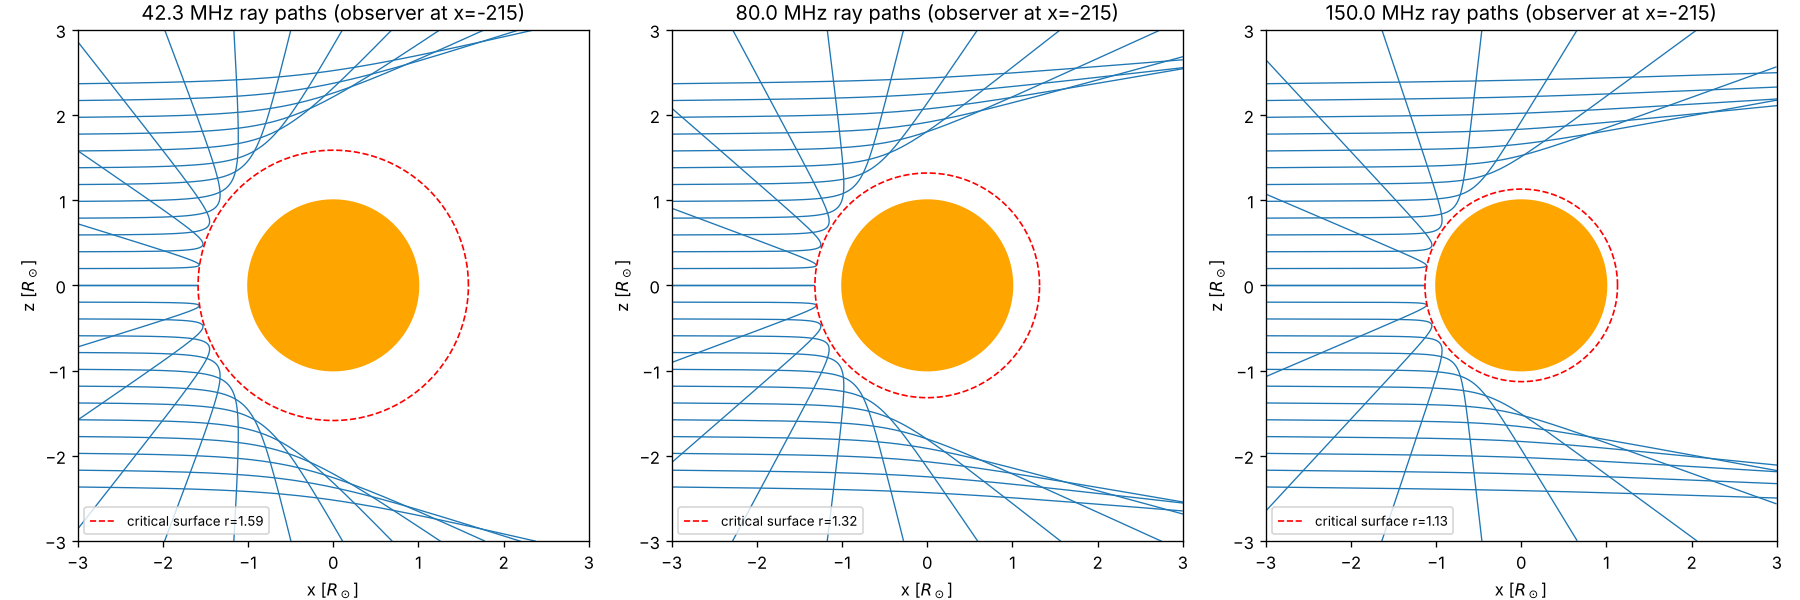
\includegraphics[width=0.92\textwidth]{fig/ray_paths.png}\par
\vspace{1.2cm}
{\Large Line-by-line Code Reference\par}\vspace{0.3cm}{\normalsize Companion to the User Manual, \code{radiosynth\_user\_manual.pdf},\\ to which the references to chapters, sections and equations point.\par}
\vfill
{\Large Soumitra Hazra\par}
\vspace{0.3cm}
{\large Second version (2.2.0) \quad---\quad November 2026\par}
\vspace{0.2cm}
{\small Free software under the GNU General Public License, version 3 or later\par}
\vspace{0.4cm}
{\small Algorithm after Benkevitch et al.\ (2010, ApJ 725, 447) and Moschou et al.\ (2018, ApJ 867, 51)\par}
\end{titlepage}

\tableofcontents

\mainmatter
\chapter*{How this document is organised}
\addcontentsline{toc}{chapter}{How this document is organised}
This document describes the source code of \code{radiosynth} line by line; how to use the package and the physics are in the User Manual. The chapters follow the folders of the package (User Manual, Section~\ref{sec:layout}): first the
common machinery (\code{radiosynth/common/}), then one group of chapters per emission
mechanism (\code{simplistic/}, \code{bremsstrahlung/}, \code{gyroresonance/}), and finally
the package files \code{\_\_init\_\_.py} and \code{\_\_main\_\_.py}. Each chapter lists the
source in blocks, with the line numbers of the file, followed by a commentary that refers
to individual lines. The listings are generated from the source files at the time the
manual is built, so the line numbers always match the distributed code. \code{radiosynth} is written by Soumitra Hazra and is
distributed under the GNU General Public License, version 3 or later; every source file
starts with the corresponding copyright and licence lines.
\chapter{common/constants.py --- physical constants}
\label{mod:common:constants.py}
\textbf{File:} \code{radiosynth/common/constants.py} --- 38 lines.

All numbers in SI units. The solar radius is the BATS-R-US value (6.96e8 m), so that
lengths in $R_\odot$ convert exactly as in the Fortran code.

\section*{\normalsize Module header and imports \hfill{\small\mdseries\color{gray}lines 4--10}}
\addcontentsline{toc}{section}{Module header and imports}
\lstinputlisting[style=py,firstline=4,lastline=10,firstnumber=4]{src/common/constants.py}
\begin{lines}
\item[L.10] \code{scipy.\allowbreak{}constants} provides CODATA values of $k_B$, $m_e$, $m_p$, $e$, $c$, $\varepsilon_0$.
\end{lines}
\section*{\normalsize Constant definitions \hfill{\small\mdseries\color{gray}lines 12--25}}
\addcontentsline{toc}{section}{Constant definitions}
\lstinputlisting[style=py,firstline=12,lastline=25,firstnumber=12]{src/common/constants.py}
\begin{lines}
\item[L.13] Boltzmann constant [J/K]; used in $B_\nu$ and in $T_e=P/(n k_B)$.
\item[L.14–17] Electron and proton masses, elementary charge, speed of light.
\item[L.20] $e^2/(4\pi\varepsilon_0)$ in J m. This is \code{cElectronChargeSquaredJm} of BATS-R-US and appears in $n_\text{cr}$ and in $\kappa_\nu$.
\item[L.21] Solar radius used to convert path lengths in $R_\odot$ to metres.
\item[L.22–23] 1 AU in metres and in solar radii (about 215); a natural observer distance.
\item[L.24–25] Flux units: 1 Jy $=10^{-26}$ and 1 sfu $=10^{-22}$ W m$^{-2}$ Hz$^{-1}$.
\end{lines}
\section*{\normalsize critical\_density() \hfill{\small\mdseries\color{gray}lines 28--33}}
\addcontentsline{toc}{section}{critical\_density()}
\lstinputlisting[style=py,firstline=28,lastline=33,firstnumber=28]{src/common/constants.py}
\begin{lines}
\item[L.33] Eq. (\ref{eq:ncr}): $n_\text{cr}=\pi m_e f^2/(e^2/4\pi\varepsilon_0)$, identical to \code{NElectronSiCr =\allowbreak{} cPi*\allowbreak{}cElectronMass*\allowbreak{}RadioFrequency*\allowbreak{}*\allowbreak{}2/\allowbreak{}cElectronChargeSquaredJm}. It accepts scalars or arrays.
\end{lines}
\section*{\normalsize plasma\_frequency() \hfill{\small\mdseries\color{gray}lines 36--38}}
\addcontentsline{toc}{section}{plasma\_frequency()}
\lstinputlisting[style=py,firstline=36,lastline=38,firstnumber=36]{src/common/constants.py}
\begin{lines}
\item[L.38] The inverse relation, $f_p=\sqrt{n_e e^2/(4\pi\varepsilon_0\,\pi m_e)}\approx 8.98\sqrt{n_e[\text{m}^{-3}]}$ Hz.
\end{lines}

\chapter{common/magnetoionic.py --- cold-plasma magneto-ionic theory}
\label{mod:common:magnetoionic.py}
\textbf{File:} \code{radiosynth/common/magnetoionic.py} --- 82 lines.

Shared by the magnetised free--free coefficients and the gyroresonance opacity: the
parameters $X$, $Y$, the axial ratio of the modes, the Appleton--Hartree refractive
index and the cutoffs.

\section*{\normalsize Module docstring and imports \hfill{\small\mdseries\color{gray}lines 4--36}}
\addcontentsline{toc}{section}{Module docstring and imports}
\lstinputlisting[style=py,firstline=4,lastline=36,firstnumber=4]{src/common/magnetoionic.py}
Defines the notation ($X$, $Y$, $\theta$ with $\vect k$ towards the observer), the modes, the Appleton--Hartree formula, the polarisation vector $(T\cos\theta,\,i,\,-T\sin\theta)/\sqrt{1+T^2}$ and the handedness convention: for $\vect B\cdot\vect k>0$ the x-mode is right-hand circularly polarised (IAU/IEEE), $V>0$.

\section*{\normalsize Gyrofrequency \hfill{\small\mdseries\color{gray}lines 37--37}}
\addcontentsline{toc}{section}{Gyrofrequency}
\lstinputlisting[style=py,firstline=37,lastline=37,firstnumber=37]{src/common/magnetoionic.py}
\begin{lines}
\item[L.37] $\nu_B=eB/(2\pi m_e)$ per gauss: 2.7992 MHz/G.
\end{lines}
\section*{\normalsize gyrofrequency() and magnetoionic\_params() \hfill{\small\mdseries\color{gray}lines 40--49}}
\addcontentsline{toc}{section}{gyrofrequency() and magnetoionic\_params()}
\lstinputlisting[style=py,firstline=40,lastline=49,firstnumber=40]{src/common/magnetoionic.py}
\begin{lines}
\item[L.47] $X=n_e/n_\text{cr}=(\nu_p/\nu)^2$ (same $n_\text{cr}$ as the ray tracer).
\item[L.48] $Y=\nu_B/\nu$.
\end{lines}
\section*{\normalsize axial\_ratio\_x() \hfill{\small\mdseries\color{gray}lines 52--60}}
\addcontentsline{toc}{section}{axial\_ratio\_x()}
\lstinputlisting[style=py,firstline=52,lastline=60,firstnumber=52]{src/common/magnetoionic.py}
\begin{lines}
\item[L.59] $|T_x|=2(1-X)|\cos\theta|/[Y\sin^2\theta+\sqrt{Y^2\sin^4\theta+4(1-X)^2\cos^2\theta}]$: 1 (circular) along $\vect B$, 0 (linear, $\vect E\perp\vect B$) across it.
\item[L.60] Guard against $0/0$ when $Y=0$ and $\cos\theta=0$.
\end{lines}
\section*{\normalsize refractive\_index2() \hfill{\small\mdseries\color{gray}lines 63--74}}
\addcontentsline{toc}{section}{refractive\_index2()}
\lstinputlisting[style=py,firstline=63,lastline=74,firstnumber=63]{src/common/magnetoionic.py}
\begin{lines}
\item[L.70–72] Appleton--Hartree with the $+$ root for the o-mode and $-$ for the x-mode: along $\vect B$, $n^2=1-X/(1\pm Y)$.
\end{lines}
\section*{\normalsize cutoff() \hfill{\small\mdseries\color{gray}lines 77--82}}
\addcontentsline{toc}{section}{cutoff()}
\lstinputlisting[style=py,firstline=77,lastline=82,firstnumber=77]{src/common/magnetoionic.py}
o-mode: $X\ge1$; x-mode: $X\ge1-Y$. The transfer stops a polarisation at its cutoff.


\chapter{common/grid.py --- model grids and interpolation}
\label{mod:common:grid.py}
\textbf{File:} \code{radiosynth/common/grid.py} --- 523 lines.

The ray tracer asks a grid object for five things at arbitrary points: $n_e$,
$\nabla n_e$, $T_e$, the local cell size, and whether the point is inside the domain.
\code{MHDGrid} (Cartesian, rectilinear) and \code{SphericalGrid} ($r,\theta,\phi$) provide the same
interface: \code{sample(\allowbreak{}p)}, \code{inside(\allowbreak{}p)}, \code{domain\_\allowbreak{}intersection(\allowbreak{}o,\allowbreak{} d)}, \code{r\_\allowbreak{}body}, \code{to\_\allowbreak{}npz(\allowbreak{})}.
This replaces BATS-R-US's \code{get\_\allowbreak{}local\_\allowbreak{}density}, \code{interpolate\_\allowbreak{}grid\_\allowbreak{}amr\_\allowbreak{}gc},
\code{calc\_\allowbreak{}gradient\_\allowbreak{}ghost} and \code{CellSize\_\allowbreak{}DB}.

\section*{\normalsize Module docstring and import \hfill{\small\mdseries\color{gray}lines 4--19}}
\addcontentsline{toc}{section}{Module docstring and import}
\lstinputlisting[style=py,firstline=4,lastline=19,firstnumber=4]{src/common/grid.py}
Explains the correspondence with the BATS-R-US interpolation routines. The density gradient is pre-computed on the grid and interpolated, exactly as BATS-R-US interpolates \code{GradVar\_\allowbreak{}DGB}.

\section*{\normalsize MHDGrid: class docstring \hfill{\small\mdseries\color{gray}lines 22--39}}
\addcontentsline{toc}{section}{MHDGrid: class docstring}
\lstinputlisting[style=py,firstline=22,lastline=39,firstnumber=22]{src/common/grid.py}
\begin{lines}
\item[L.39] Five fields are stored per grid point, interleaved in one array: $n_e$, $\partial_x n_e$, $\partial_y n_e$, $\partial_z n_e$, $T_e$. Interleaving means one memory fetch per cell corner returns all five values.
\end{lines}
\section*{\normalsize MHDGrid.\_\_init\_\_: input checks \hfill{\small\mdseries\color{gray}lines 41--58}}
\addcontentsline{toc}{section}{MHDGrid.\_\_init\_\_: input checks}
\lstinputlisting[style=py,firstline=41,lastline=58,firstnumber=41]{src/common/grid.py}
\begin{lines}
\item[L.42–44] Axes as float arrays (in $R_\odot$).
\item[L.45–47] Each axis must be 1D, strictly increasing and have at least two points; otherwise interpolation is undefined.
\item[L.48–51] The density must be shaped (nx, ny, nz) in \code{ij} ordering, the same order as the axes.
\item[L.52] NaN or infinite values become 0 and negative densities are clipped to 0. This guards against ghost-cell or undefined values in model output.
\item[L.53–58] Temperature is optional (not needed for the simplistic mechanism); it defaults to 1 K. Non-finite values become 1 K.
\end{lines}
\section*{\normalsize MHDGrid.\_\_init\_\_: gradient and storage \hfill{\small\mdseries\color{gray}lines 60--72}}
\addcontentsline{toc}{section}{MHDGrid.\_\_init\_\_: gradient and storage}
\lstinputlisting[style=py,firstline=60,lastline=72,firstnumber=60]{src/common/grid.py}
\begin{lines}
\item[L.61] Inner boundary radius: a ray stops when it reaches it (BATS-R-US \code{IsBody}).
\item[L.62] Metres per coordinate unit: $R_\odot$ by default, $R_\ast$ for stellar models. The tracer converts path lengths with it.
\item[L.64] Density gradient with second-order central differences in the interior and second-order one-sided differences at the edges. Works for non-uniform axes. The unit is m$^{-3}$ per $R_\odot$, matching positions in $R_\odot$.
\item[L.65–70] Fill the interleaved array, by default in float32 to halve memory (5 fields $\times$ 4 bytes per point).
\item[L.71] Flatten to (Npoints, 5) so that a single integer index addresses a grid point.
\item[L.72] Free the temporary arrays.
\end{lines}
\section*{\normalsize MHDGrid.\_\_init\_\_: helpers for fast lookup \hfill{\small\mdseries\color{gray}lines 73--85}}
\addcontentsline{toc}{section}{MHDGrid.\_\_init\_\_: helpers for fast lookup}
\lstinputlisting[style=py,firstline=73,lastline=85,firstnumber=73]{src/common/grid.py}
\begin{lines}
\item[L.73–75] Cell widths along each axis; used for interpolation weights and the local cell size.
\item[L.76–77] Corners of the domain box.
\item[L.78] If all three axes are uniform, locating a cell is a division (\code{floor}) rather than a binary search.
\item[L.79] Flat-index strides for C-ordered (nx, ny, nz) arrays: index $=i\,n_yn_z+j\,n_z+k$.
\item[L.80–85] Pre-compute the 8 flat-index offsets of the cell corners $(i+d_i, j+d_j, k+d_k)$, $d\in\{0,1\}$.
\end{lines}
\section*{\normalsize MHDGrid: properties \hfill{\small\mdseries\color{gray}lines 87--99}}
\addcontentsline{toc}{section}{MHDGrid: properties}
\lstinputlisting[style=py,firstline=87,lastline=99,firstnumber=87]{src/common/grid.py}
\begin{lines}
\item[L.89] Memory used by the stored fields.
\item[L.92] One-line description printed by the driver (shape, extent, smallest cell, $r_\text{body}$).
\item[L.98] Smallest cell width over all axes.
\end{lines}
\section*{\normalsize MHDGrid.inside() \hfill{\small\mdseries\color{gray}lines 101--103}}
\addcontentsline{toc}{section}{MHDGrid.inside()}
\lstinputlisting[style=py,firstline=101,lastline=103,firstnumber=101]{src/common/grid.py}
\begin{lines}
\item[L.103] A point is inside if all three coordinates lie within $[\text{lo},\text{hi}]$. Vectorised over N points.
\end{lines}
\section*{\normalsize MHDGrid.\_locate(): find the cell and the fractional position \hfill{\small\mdseries\color{gray}lines 105--112}}
\addcontentsline{toc}{section}{MHDGrid.\_locate(): find the cell and the fractional position}
\lstinputlisting[style=py,firstline=105,lastline=112,firstnumber=105]{src/common/grid.py}
\begin{lines}
\item[L.106–107] Uniform axis: $i=\lfloor(u-x_0)/\Delta x\rfloor$.
\item[L.109] Non-uniform axis: binary search, $O(\log n)$ per point.
\item[L.110] Clip to valid cells $[0,n-2]$; points outside are evaluated at the boundary value.
\item[L.111–112] Fractional position $t\in[0,1]$ inside the cell, used as the linear weight.
\end{lines}
\section*{\normalsize MHDGrid.sample(): trilinear interpolation \hfill{\small\mdseries\color{gray}lines 114--144}}
\addcontentsline{toc}{section}{MHDGrid.sample(): trilinear interpolation}
\lstinputlisting[style=py,firstline=114,lastline=144,firstnumber=114]{src/common/grid.py}
\begin{lines}
\item[L.126] Domain flag returned to the tracer.
\item[L.127–129] Cell indices and weights along x, y, z.
\item[L.130] Flat index of the lower corner of each point's cell.
\item[L.131–134] Accumulator for the 5 fields, and the linear weights $(1-t, t)$ along each axis.
\item[L.136–142] Sum over the 8 corners: weight $w=w_x w_y w_z$ times the corner's 5 field values. Each step gathers N rows of the field table at once. This is the trilinear interpolation of BATS-R-US (\code{Weight\_\allowbreak{}I} in \code{get\_\allowbreak{}local\_\allowbreak{}density}).
\item[L.143] Local cell size $\min(\Delta x,\Delta y,\Delta z)$: the target step \code{DeltaSNew}.
\item[L.144] Return $n_e$ (clipped $\ge0$), $\nabla n_e$ (N,3), $T_e$, cell size and the inside flag.
\end{lines}
\section*{\normalsize MHDGrid: magnetic field \hfill{\small\mdseries\color{gray}lines 146--197}}
\addcontentsline{toc}{section}{MHDGrid: magnetic field}
\lstinputlisting[style=py,firstline=146,lastline=197,firstnumber=146]{src/common/grid.py}
The field is optional and stored separately from $n_e$ and $T_e$, so grids without a field use no extra memory and the refractive tracer is unchanged.

\begin{lines}
\item[L.148] True once a field has been attached.
\item[L.151–157] Stack $(B_x,B_y,B_z)$ [G] on the grid nodes, check the shape, replace non-finite values by 0 and keep them in \code{float32} as a (N,3) array.
\item[L.160–175] Generic trilinear interpolation of any (nodes, k) array, with the same cell location and the same eight weights as \code{sample(\allowbreak{})}.
\item[L.177] $\vect B$ [G] at the points, Cartesian components.
\item[L.185–193] Any named scalar field on the nodes (stored in \code{grid.\allowbreak{}scalars}), e.g. the current density \code{'j'} (common/fields.py), for use in fast-electron rules.
\item[L.195] Its value at the points.
\end{lines}
\section*{\normalsize MHDGrid.box\_intersection(): where a straight ray enters and leaves the box \hfill{\small\mdseries\color{gray}lines 199--215}}
\addcontentsline{toc}{section}{MHDGrid.box\_intersection(): where a straight ray enters and leaves the box}
\lstinputlisting[style=py,firstline=199,lastline=215,firstnumber=199]{src/common/grid.py}
Slab method: for each axis, the ray $\vect o+t\vect d$ is between the two faces for $t\in[t_1,t_2]$; the intersection over the three axes is $[\max t_\text{min},\min t_\text{max}]$.

\begin{lines}
\item[L.204] Same observer for all rays (broadcast).
\item[L.205–206] Avoid division by zero for directions parallel to a face.
\item[L.207–210] Face crossings along each axis.
\item[L.212–214] Parallel rays are either always inside that slab ($\pm\infty$) or never (empty interval).
\item[L.215] Entry and exit parameters; the ray misses if exit $<$ entry.
\end{lines}
\section*{\normalsize MHDGrid: common API \hfill{\small\mdseries\color{gray}lines 217--236}}
\addcontentsline{toc}{section}{MHDGrid: common API}
\lstinputlisting[style=py,firstline=217,lastline=236,firstnumber=217]{src/common/grid.py}
\begin{lines}
\item[L.218] Generic name used by \code{image.\allowbreak{}start\_\allowbreak{}points}, so Cartesian and spherical grids are interchangeable.
\item[L.231] Largest radius inside the box; used to start parallel rays outside the model.
\item[L.220–227] Save $n_e$, $T_e$ and the axes. \code{load\_\allowbreak{}mhd(\allowbreak{}'file.\allowbreak{}npz')} rebuilds the grid without re-reading the original model.
\end{lines}
\section*{\normalsize SphericalGrid: class docstring \hfill{\small\mdseries\color{gray}lines 237--260}}
\addcontentsline{toc}{section}{SphericalGrid: class docstring}
\lstinputlisting[style=py,firstline=237,lastline=260,firstnumber=237]{src/common/grid.py}
Used for PLUTO (and any) spherical output. Sampling is done in $(r,\theta,\phi)$ index space, so the stretched radial grid near the Sun is used as is.

\begin{lines}
\item[L.260] Stored fields: $n_e$, $\partial_r n_e$, $r^{-1}\partial_\theta n_e$, $(r\sin\theta)^{-1}\partial_\phi n_e$, $T_e$. These are the spherical components of the gradient vector, converted to Cartesian after interpolation.
\end{lines}
\section*{\normalsize SphericalGrid.\_\_init\_\_: fields \hfill{\small\mdseries\color{gray}lines 262--273}}
\addcontentsline{toc}{section}{SphericalGrid.\_\_init\_\_: fields}
\lstinputlisting[style=py,firstline=262,lastline=273,firstnumber=262]{src/common/grid.py}
\begin{lines}
\item[L.266] A single (or absent) $\phi$ value means a 2.5D axisymmetric model.
\item[L.267] Store at least one $\phi$ value so the array is always 3D.
\item[L.269–272] Reshape to (nr, nth, nph) and clean invalid values, as in \code{MHDGrid}.
\end{lines}
\section*{\normalsize SphericalGrid.\_\_init\_\_: domain extent \hfill{\small\mdseries\color{gray}lines 275--291}}
\addcontentsline{toc}{section}{SphericalGrid.\_\_init\_\_: domain extent}
\lstinputlisting[style=py,firstline=275,lastline=291,firstnumber=275]{src/common/grid.py}
\begin{lines}
\item[L.275–281] Use the given cell edges, or reconstruct them as mid-points between centres plus half a cell at each end.
\item[L.284] Colatitude edges are limited to $[0,\pi]$.
\item[L.286] Inner and outer radii of the domain.
\item[L.287] Does the grid cover the whole colatitude range? If not, rays leaving the wedge stop.
\item[L.288–289] Full $2\pi$ in longitude (or axisymmetric) means $\phi$ is periodic.
\item[L.290] Rays stop at the inner boundary, by default the inner radial edge (usually 1 $R_\odot$).
\end{lines}
\section*{\normalsize SphericalGrid.\_\_init\_\_: gradient components \hfill{\small\mdseries\color{gray}lines 293--316}}
\addcontentsline{toc}{section}{SphericalGrid.\_\_init\_\_: gradient components}
\lstinputlisting[style=py,firstline=293,lastline=316,firstnumber=293]{src/common/grid.py}
\begin{lines}
\item[L.294–295] Broadcast helpers $r$ and $\sin\theta$ ($\ge10^{-6}$ to avoid division by zero at the poles).
\item[L.296] $\partial n_e/\partial r$.
\item[L.297–298] $r^{-1}\partial n_e/\partial\theta$.
\item[L.300–303] Periodic $\phi$: pad one cell on each side with the wrapped values so that the central difference is correct at $\phi=0$ and $2\pi$.
\item[L.305] Non-periodic wedge: ordinary one-sided differences at the edges.
\item[L.306] $(r\sin\theta)^{-1}\partial n_e/\partial\phi$.
\item[L.308] Axisymmetric: no $\phi$ gradient.
\item[L.309–311] Interleaved storage as in \code{MHDGrid}.
\item[L.313–315] Cell widths in $r$, $\theta$, $\phi$ (used for the step size).
\item[L.316] Flat-index strides for the (nr, nth, nph) array.
\end{lines}
\section*{\normalsize SphericalGrid: description and properties \hfill{\small\mdseries\color{gray}lines 318--334}}
\addcontentsline{toc}{section}{SphericalGrid: description and properties}
\lstinputlisting[style=py,firstline=318,lastline=334,firstnumber=318]{src/common/grid.py}
\begin{lines}
\item[L.319] Reports whether the model is axisymmetric or 3D, and its extent in degrees.
\item[L.331] Smallest of $\Delta r$ and $r_\text{lo}\Delta\theta$.
\end{lines}
\section*{\normalsize SphericalGrid.\_sph(): Cartesian to spherical \hfill{\small\mdseries\color{gray}lines 335--339}}
\addcontentsline{toc}{section}{SphericalGrid.\_sph(): Cartesian to spherical}
\lstinputlisting[style=py,firstline=335,lastline=339,firstnumber=335]{src/common/grid.py}
\begin{lines}
\item[L.336] $r=|\vect p|$.
\item[L.337] Colatitude $\theta=\arccos(z/r)$ (clipped for round-off).
\item[L.338] Longitude $\phi=\operatorname{atan2}(y,x)$ mapped to $[0,2\pi)$.
\end{lines}
\section*{\normalsize SphericalGrid.\_phi\_rel() and inside() \hfill{\small\mdseries\color{gray}lines 341--355}}
\addcontentsline{toc}{section}{SphericalGrid.\_phi\_rel() and inside()}
\lstinputlisting[style=py,firstline=341,lastline=355,firstnumber=341]{src/common/grid.py}
\begin{lines}
\item[L.343] Longitude measured from the first edge, so a wedge starting at any angle can be tested with one comparison.
\item[L.347] Inside the radial shell ...
\item[L.348] ... and within the colatitude range, if limited ...
\item[L.350] ... and within the longitude range, if limited.
\end{lines}
\section*{\normalsize SphericalGrid.\_locate() \hfill{\small\mdseries\color{gray}lines 356--362}}
\addcontentsline{toc}{section}{SphericalGrid.\_locate()}
\lstinputlisting[style=py,firstline=356,lastline=362,firstnumber=356]{src/common/grid.py}
\begin{lines}
\item[L.358] A single cell (axisymmetric $\phi$): index 0, weight 0.
\item[L.360–361] Binary search for the bracketing cell centres and the linear weight. The spherical axes are often stretched, so no uniform shortcut is used.
\end{lines}
\section*{\normalsize SphericalGrid.sample(): locate in r and theta \hfill{\small\mdseries\color{gray}lines 364--372}}
\addcontentsline{toc}{section}{SphericalGrid.sample(): locate in r and theta}
\lstinputlisting[style=py,firstline=364,lastline=372,firstnumber=364]{src/common/grid.py}
\begin{lines}
\item[L.366] Spherical coordinates of the sample points.
\item[L.367–369] Domain flag (radial shell, colatitude range).
\item[L.370–371] Bracketing indices and weights in $r$ and $\theta$.
\end{lines}
\section*{\normalsize SphericalGrid.sample(): longitude handling \hfill{\small\mdseries\color{gray}lines 373--390}}
\addcontentsline{toc}{section}{SphericalGrid.sample(): longitude handling}
\lstinputlisting[style=py,firstline=373,lastline=390,firstnumber=373]{src/common/grid.py}
\begin{lines}
\item[L.373–376] Axisymmetric: both $\phi$ corners are the single cell, so the field does not depend on $\phi$.
\item[L.377–385] Periodic longitude: the last cell centre is followed by the first one plus $2\pi$. \code{k1 =\allowbreak{} (\allowbreak{}k0+1) \% nph} wraps around, and the weight uses a $2\pi$-shifted upper centre.
\item[L.386–390] Limited wedge: ordinary search; points outside the wedge are flagged.
\end{lines}
\section*{\normalsize SphericalGrid.sample(): trilinear interpolation in index space \hfill{\small\mdseries\color{gray}lines 391--399}}
\addcontentsline{toc}{section}{SphericalGrid.sample(): trilinear interpolation in index space}
\lstinputlisting[style=py,firstline=391,lastline=399,firstnumber=391]{src/common/grid.py}
\begin{lines}
\item[L.393–399] Weighted sum over the 8 corner cells. \code{np.\allowbreak{}minimum(\allowbreak{}.\allowbreak{}.\allowbreak{}.\allowbreak{},\allowbreak{} size-1)} keeps the upper index valid when a point is beyond the last centre; the weight is then zero.
\end{lines}
\section*{\normalsize SphericalGrid.sample(): gradient to Cartesian, cell size \hfill{\small\mdseries\color{gray}lines 400--413}}
\addcontentsline{toc}{section}{SphericalGrid.sample(): gradient to Cartesian, cell size}
\lstinputlisting[style=py,firstline=400,lastline=413,firstnumber=400]{src/common/grid.py}
\begin{lines}
\item[L.400–402] Unpack the interpolated fields and the trigonometric factors at each point.
\item[L.403–406] Transform $(g_r,g_\theta,g_\phi)$ to Cartesian with the unit vectors $\hat r=(s_\theta c_\phi, s_\theta s_\phi, c_\theta)$, $\hat\theta=(c_\theta c_\phi, c_\theta s_\phi, -s_\theta)$, $\hat\phi=(-s_\phi, c_\phi, 0)$.
\item[L.407–409] Local cell size $\min(\Delta r, r\Delta\theta)$.
\item[L.410–412] Include $r\sin\theta\,\Delta\phi$ in 3D, floored at a quarter of $r\Delta\theta$. The cells near the poles are tiny, and without the floor the step size would collapse there.
\item[L.413] Same return signature as \code{MHDGrid.\allowbreak{}sample}.
\end{lines}
\section*{\normalsize SphericalGrid: magnetic field \hfill{\small\mdseries\color{gray}lines 415--493}}
\addcontentsline{toc}{section}{SphericalGrid: magnetic field}
\lstinputlisting[style=py,firstline=415,lastline=493,firstnumber=415]{src/common/grid.py}
\begin{lines}
\item[L.420–431] The field is given at the cell centres either as spherical components $(B_r,B_\theta,B_\phi)$ --- PLUTO's \code{bx1}, \code{bx2}, \code{bx3} --- or as Cartesian components. The choice is remembered in \code{\_\allowbreak{}bcomp}.
\item[L.434–464] Generic interpolation in $(r,\theta,\phi)$ index space of any (cells, k) array, with the same longitude handling as \code{sample(\allowbreak{})} (axisymmetric, periodic, or a longitude patch); also returns $\theta$, $\phi$ of the points.
\item[L.466–473] $\vect B$ at the points; Cartesian components are returned as they are.
\item[L.474–481] Spherical to Cartesian at the sample point: $B_x=B_r\sin\theta\cos\phi+B_\theta\cos\theta\cos\phi-B_\phi\sin\phi$, and similarly for $B_y$, $B_z$. Interpolating the spherical components and rotating afterwards keeps a radial field radial between grid points.
\item[L.483–491] Named scalar fields at the cell centres, as for the Cartesian grid.
\end{lines}
\section*{\normalsize SphericalGrid.domain\_intersection() \hfill{\small\mdseries\color{gray}lines 495--507}}
\addcontentsline{toc}{section}{SphericalGrid.domain\_intersection()}
\lstinputlisting[style=py,firstline=495,lastline=507,firstnumber=495]{src/common/grid.py}
\begin{lines}
\item[L.499–501] Solve $|\vect o+t\vect d|=r_\text{hi}$: $t=-b\pm\sqrt{b^2-c}$, with $b=\vect o\cdot\vect d$ and $c=|\vect o|^2-r_\text{hi}^2$.
\item[L.503–504] Entry and exit; rays that miss the sphere get an empty interval.
\item[L.507] Alias for symmetry with \code{MHDGrid}.
\end{lines}
\section*{\normalsize SphericalGrid.to\_npz() \hfill{\small\mdseries\color{gray}lines 509--523}}
\addcontentsline{toc}{section}{SphericalGrid.to\_npz()}
\lstinputlisting[style=py,firstline=509,lastline=523,firstnumber=509]{src/common/grid.py}
Saves everything needed to rebuild the grid, including the \code{geometry=\allowbreak{}'spherical'} tag that \code{load\_\allowbreak{}mhd} checks.


\chapter{common/readers.py --- BATS-R-US and generic input}
\label{mod:common:readers.py}
\textbf{File:} \code{radiosynth/common/readers.py} --- 567 lines.

Turns model files into dictionaries of point variables, works out $n_e$ and $T_e$
with the right units, arranges the points on a grid (or resamples them), and returns an
\code{MHDGrid}. \code{load\_\allowbreak{}mhd} is the single entry point and also dispatches to the PLUTO
reader.

\section*{\normalsize Module docstring and imports \hfill{\small\mdseries\color{gray}lines 4--35}}
\addcontentsline{toc}{section}{Module docstring and imports}
\lstinputlisting[style=py,firstline=4,lastline=35,firstnumber=4]{src/common/readers.py}
Lists the supported formats. Every reader returns \code{\{name: array\}}, which \code{build\_\allowbreak{}grid} converts.

\section*{\normalsize Variable-name helpers \hfill{\small\mdseries\color{gray}lines 36--51}}
\addcontentsline{toc}{section}{Variable-name helpers}
\lstinputlisting[style=py,firstline=36,lastline=51,firstnumber=36]{src/common/readers.py}
\begin{lines}
\item[L.36] Base name in lower case: \code{'Rho [g/\allowbreak{}cm\^{}3]'} becomes \code{'rho'}.
\item[L.41] Unit in square brackets, lower case without spaces: \code{'g/\allowbreak{}cm\^{}3'}.
\item[L.46] First variable whose base name is in the candidate list.
\end{lines}
\section*{\normalsize Unit tables \hfill{\small\mdseries\color{gray}lines 54--59}}
\addcontentsline{toc}{section}{Unit tables}
\lstinputlisting[style=py,firstline=54,lastline=59,firstnumber=54]{src/common/readers.py}
\begin{lines}
\item[L.54] Mass-density units and their factor to kg m$^{-3}$.
\item[L.55] Number-density units and their factor to m$^{-3}$. BATS-R-US 'amu/cc' and 'Mp/cc' are number densities.
\item[L.58] Pressure units and their factor to Pa (1 dyn cm$^{-2}$ = 0.1 Pa).
\end{lines}
\section*{\normalsize find\_magnetic\_field(): Bx, By, Bz in gauss \hfill{\small\mdseries\color{gray}lines 62--91}}
\addcontentsline{toc}{section}{find\_magnetic\_field(): Bx, By, Bz in gauss}
\lstinputlisting[style=py,firstline=62,lastline=91,firstnumber=62]{src/common/readers.py}
\begin{lines}
\item[L.62] Gauss per unit: G = 1, nT = $10^{-5}$, T = $10^4$, mT = 10.
\item[L.71–75] Look for \code{Bx,\allowbreak{} By,\allowbreak{} Bz}, then \code{B\_\allowbreak{}x,\allowbreak{} .\allowbreak{}.\allowbreak{}.\allowbreak{}}, then \code{b1,\allowbreak{} b2,\allowbreak{} b3} (names compared without units and case).
\item[L.79–81] An explicit \code{b\_\allowbreak{}unit} wins: a number (gauss per file unit) or a unit name.
\item[L.83–88] Otherwise the unit in the variable name (e.g. \code{Bx [Gauss]}, BATS-R-US Tecplot) is used; without one, gauss is assumed with a warning. BATS-R-US IDL files in normalised units need \code{b\_\allowbreak{}unit}.
\end{lines}
\section*{\normalsize \_density\_to\_ne(): density in any unit to n\_e \hfill{\small\mdseries\color{gray}lines 94--120}}
\addcontentsline{toc}{section}{\_density\_to\_ne(): density in any unit to n\_e}
\lstinputlisting[style=py,firstline=94,lastline=120,firstnumber=94]{src/common/readers.py}
\begin{lines}
\item[L.101–102] Mass density: $n_e=\rho/(\mu m_p)$.
\item[L.103–104] Number density: unit conversion only.
\item[L.106–110] Unknown unit: take the median value at $r=1.05$--$1.3\,R_\odot$ as reference.
\item[L.111–119] Try g/cm$^3$, kg/m$^3$, cm$^{-3}$ and m$^{-3}$ (or only the mass or number options if the name says which) and pick the one that gives $n_e$ closest to $10^{14.5}$ m$^{-3}$, a typical low-corona value. The choice is printed, so you can check it.
\end{lines}
\section*{\normalsize \_pressure\_si() \hfill{\small\mdseries\color{gray}lines 123--127}}
\addcontentsline{toc}{section}{\_pressure\_si()}
\lstinputlisting[style=py,firstline=123,lastline=127,firstnumber=123]{src/common/readers.py}
\begin{lines}
\item[L.127] Without a recognised unit, the BATS-R-US dimensional default dyn cm$^{-2}$ is assumed.
\end{lines}
\section*{\normalsize derive\_ne\_te(): electron density \hfill{\small\mdseries\color{gray}lines 130--150}}
\addcontentsline{toc}{section}{derive\_ne\_te(): electron density}
\lstinputlisting[style=py,firstline=130,lastline=150,firstnumber=130]{src/common/readers.py}
\begin{lines}
\item[L.138] Radius of every point, for the unit guess and the printed check.
\item[L.140] Density variable: user choice or the first of ne, n\_e, rho, n, dens, density.
\item[L.143–145] Unit: from the user, from the name, or from the IDL header units.
\item[L.146–148] If there is no unit, the name decides whether it is a mass or a number density.
\item[L.149] Convert to m$^{-3}$ and remember how, for the report.
\end{lines}
\section*{\normalsize derive\_ne\_te(): electron temperature \hfill{\small\mdseries\color{gray}lines 152--192}}
\addcontentsline{toc}{section}{derive\_ne\_te(): electron temperature}
\lstinputlisting[style=py,firstline=152,lastline=192,firstnumber=152]{src/common/readers.py}
\begin{lines}
\item[L.154–157] 1st choice: a Te variable in K.
\item[L.159–162] 2nd: electron pressure, $T_e=P_e/(n_ek_B)$ (AWSoM writes Pe).
\item[L.165–168] 3rd: total pressure, $T=P/(2n_ek_B)$, i.e. $T_e=T_i$ in a hydrogen plasma.
\item[L.171] 4th: a generic temperature variable.
\item[L.176–178] Last: a constant given by the user, otherwise an error.
\item[L.180–186] Print what was used and the median $n_e$, $T_e$ near $r=1.1\,R_\odot$. This is the best check that the units are right.
\end{lines}
\section*{\normalsize \_unique\_axis() \hfill{\small\mdseries\color{gray}lines 193--202}}
\addcontentsline{toc}{section}{\_unique\_axis()}
\lstinputlisting[style=py,firstline=193,lastline=202,firstnumber=193]{src/common/readers.py}
\begin{lines}
\item[L.195–197] Round coordinates to a relative tolerance of $10^{-6}$ and find the distinct values. This copes with single-precision round-off in the file.
\item[L.199–201] Each axis value is the mean of the coordinates in its group; \code{inv} maps every point to its axis index.
\end{lines}
\section*{\normalsize points\_to\_grid(): tensor grid or resampling \hfill{\small\mdseries\color{gray}lines 205--229}}
\addcontentsline{toc}{section}{points\_to\_grid(): tensor grid or resampling}
\lstinputlisting[style=py,firstline=205,lastline=229,firstnumber=205]{src/common/readers.py}
\begin{lines}
\item[L.217–220] Distinct coordinate values along each axis.
\item[L.221–229] If the number of points equals $n_xn_yn_z$ and no two points share a cell, the data already form a tensor grid. They are placed by index, so any point order works (Tecplot I-fastest, shuffled, etc.).
\end{lines}
\section*{\normalsize points\_to\_grid(): resampling scattered points \hfill{\small\mdseries\color{gray}lines 231--266}}
\addcontentsline{toc}{section}{points\_to\_grid(): resampling scattered points}
\lstinputlisting[style=py,firstline=231,lastline=266,firstnumber=231]{src/common/readers.py}
\begin{lines}
\item[L.232–239] Target uniform grid (default $160^3$) over the given or full box.
\item[L.244–245] Source points and target points.
\item[L.247–251] The density is interpolated as $\log n_e$: it varies over many orders of magnitude, and linear interpolation of the logarithm keeps it positive and smooth.
\item[L.252–254] Fast nearest-neighbour lookup with a k-d tree.
\item[L.256–261] Linear interpolation on the Delaunay triangulation; target points outside the convex hull fall back to the nearest neighbour.
\item[L.262–265] Undo the logarithm and reshape to 3D.
\end{lines}
\section*{\normalsize build\_grid() and grid\_from\_arrays() \hfill{\small\mdseries\color{gray}lines 269--301}}
\addcontentsline{toc}{section}{build\_grid() and grid\_from\_arrays()}
\lstinputlisting[style=py,firstline=269,lastline=301,firstnumber=269]{src/common/readers.py}
\begin{lines}
\item[L.278] Physical fields at the points.
\item[L.284] Arrange or resample.
\item[L.286] Build the grid and attach the conversion info. With \code{r\_\allowbreak{}star} (in $R_\odot$) the coordinates are taken to be in stellar radii, as in BATS-R-US stellar runs, and the length unit is $R_\ast$.
\item[L.294] Convenience wrapper around \code{MHDGrid}.
\end{lines}
\section*{\normalsize \_standardise\_xyz() \hfill{\small\mdseries\color{gray}lines 302--310}}
\addcontentsline{toc}{section}{\_standardise\_xyz()}
\lstinputlisting[style=py,firstline=302,lastline=310,firstnumber=302]{src/common/readers.py}
\begin{lines}
\item[L.304] Make sure the coordinates are available as plain 'x', 'y', 'z', whatever their original names (for example 'X [R]').
\end{lines}
\section*{\normalsize read\_tecplot\_ascii() \hfill{\small\mdseries\color{gray}lines 313--373}}
\addcontentsline{toc}{section}{read\_tecplot\_ascii()}
\lstinputlisting[style=py,firstline=313,lastline=373,firstnumber=313]{src/common/readers.py}
\begin{lines}
\item[L.321–327] Variable names from the VARIABLES line, quoted or not, possibly over several lines.
\item[L.328–333] Select the requested zone.
\item[L.335–342] The zone header runs until the first line that starts with a number.
\item[L.344–350] Read I, J, K (ordered zone) or N, E (finite-element zone) from the header.
\item[L.351] BLOCK packing stores one variable after another; POINT packing stores one point after another.
\item[L.352] Number of points.
\item[L.354–361] Parse all numbers in one go (Fortran 'D' exponents accepted). The connectivity list of FE zones, which follows the data, is ignored.
\item[L.365] Arrange as (variable, point) for either packing.
\end{lines}
\section*{\normalsize read\_pytecplot() \hfill{\small\mdseries\color{gray}lines 374--385}}
\addcontentsline{toc}{section}{read\_pytecplot()}
\lstinputlisting[style=py,firstline=374,lastline=385,firstnumber=374]{src/common/readers.py}
\begin{lines}
\item[L.377] The same call as in the original script \code{Radio\_\allowbreak{}Emsssion\_\allowbreak{}Calculation\_\allowbreak{}batsrus.\allowbreak{}py}. Every variable of the zone is read as a NumPy array.
\end{lines}
\section*{\normalsize \_read\_records(): Fortran unformatted files \hfill{\small\mdseries\color{gray}lines 386--404}}
\addcontentsline{toc}{section}{\_read\_records(): Fortran unformatted files}
\lstinputlisting[style=py,firstline=386,lastline=404,firstnumber=386]{src/common/readers.py}
Fortran sequential files wrap every record in 4-byte length markers. The endianness is found from the first record, whose leading and trailing markers must agree.

\begin{lines}
\item[L.401–403] Split the file into records.
\end{lines}
\section*{\normalsize read\_batsrus\_idl(): binary IDL files \hfill{\small\mdseries\color{gray}lines 407--448}}
\addcontentsline{toc}{section}{read\_batsrus\_idl(): binary IDL files}
\lstinputlisting[style=py,firstline=407,lastline=448,firstnumber=407]{src/common/readers.py}
\begin{lines}
\item[L.414–419] Binary if the first 4 bytes form a plausible record length; ASCII files start with text.
\item[L.423] Record 1: header line (often the units).
\item[L.424–429] Record 2: nstep, time, ndim, npar, nvar. Its length gives the real size (4 bytes for real4, 8 for real8).
\item[L.430] Negative ndim means generalised (unstructured) coordinates.
\item[L.432] Record 3: grid dimensions.
\item[L.435–437] Record 4 (if present): equation parameters (gamma, rbody, ...).
\item[L.438] Next: names of coordinates, variables and parameters.
\item[L.442–443] Coordinates, stored in Fortran order as (point, dimension).
\item[L.446–447] One record per variable.
\end{lines}
\section*{\normalsize read\_batsrus\_idl(): ASCII files and units \hfill{\small\mdseries\color{gray}lines 449--494}}
\addcontentsline{toc}{section}{read\_batsrus\_idl(): ASCII files and units}
\lstinputlisting[style=py,firstline=449,lastline=494,firstnumber=449]{src/common/readers.py}
\begin{lines}
\item[L.451–461] ASCII layout: the same header items on lines, then one row per point.
\item[L.465–471] Name the coordinate and variable arrays.
\item[L.473–479] If the header line lists one unit per coordinate and variable (for example 'R R R g/cm3 km/s ...'), attach them as \code{\_\allowbreak{}units}.
\item[L.481] Keep the header information.
\item[L.484–490] Only 3D Cartesian coordinates are accepted here; spherical models go through \code{SphericalGrid}.
\end{lines}
\section*{\normalsize load\_mhd(): the general entry point \hfill{\small\mdseries\color{gray}lines 495--567}}
\addcontentsline{toc}{section}{load\_mhd(): the general entry point}
\lstinputlisting[style=py,firstline=495,lastline=567,firstnumber=495]{src/common/readers.py}
\begin{lines}
\item[L.508–510] A directory containing grid.out, or a .vtk file, is PLUTO output.
\item[L.511–520] Pass only the PLUTO-relevant keywords to \code{load\_\allowbreak{}pluto}.
\item[L.521–528] Drop the PLUTO keywords and unset values for the other readers.
\item[L.530] Choose the reader from the file extension.
\item[L.533–538] Call the reader.
\item[L.539–563] A saved grid is rebuilt directly (spherical or Cartesian); any other npz is treated as point data.
\item[L.566–567] Flatten the arrays and build the grid.
\end{lines}

\chapter{common/pluto.py --- PLUTO input}
\label{mod:common:pluto.py}
\textbf{File:} \code{radiosynth/common/pluto.py} --- 512 lines.

Reads PLUTO binary (\code{.\allowbreak{}dbl}/\code{.\allowbreak{}flt}) and legacy VTK output, converts code units to
physical units using \code{definitions.\allowbreak{}h}, and returns a \code{SphericalGrid} or \code{MHDGrid}.

\section*{\normalsize Module docstring \hfill{\small\mdseries\color{gray}lines 4--46}}
\addcontentsline{toc}{section}{Module docstring}
\lstinputlisting[style=py,firstline=4,lastline=46,firstnumber=4]{src/common/pluto.py}
Documents the supported formats, the unit conversion and the plasma model ($n_e$, $T$).

\section*{\normalsize PLUTO constants and default units \hfill{\small\mdseries\color{gray}lines 47--63}}
\addcontentsline{toc}{section}{PLUTO constants and default units}
\lstinputlisting[style=py,firstline=47,lastline=63,firstnumber=47]{src/common/pluto.py}
\begin{lines}
\item[L.47] The physical constants of PLUTO's \code{pluto.\allowbreak{}h} (cgs), so that \code{definitions.\allowbreak{}h} expressions such as \code{CONST\_\allowbreak{}mp*\allowbreak{}1.\allowbreak{}e8} evaluate exactly as in PLUTO.
\item[L.58] PLUTO's defaults when \code{definitions.\allowbreak{}h} does not set them: $U_\rho=m_p$, $U_L=$ 1 AU, $U_v=$ 1 km/s.
\end{lines}
\section*{\normalsize parse\_definitions() \hfill{\small\mdseries\color{gray}lines 64--83}}
\addcontentsline{toc}{section}{parse\_definitions()}
\lstinputlisting[style=py,firstline=64,lastline=83,firstnumber=64]{src/common/pluto.py}
\begin{lines}
\item[L.67–68] Evaluation namespace: the constants plus a few math functions.
\item[L.72] Match \code{\#define NAME expression} lines (a trailing C comment is ignored).
\item[L.77–79] Evaluate the expression without Python built-ins. Non-numeric defines (such as \code{PHYSICS MHD}) fail and are skipped.
\item[L.81–82] Numeric results are stored and become available to later defines.
\end{lines}
\section*{\normalsize read\_grid\_out() \hfill{\small\mdseries\color{gray}lines 86--114}}
\addcontentsline{toc}{section}{read\_grid\_out()}
\lstinputlisting[style=py,firstline=86,lastline=114,firstnumber=86]{src/common/pluto.py}
\begin{lines}
\item[L.93–96] Skip the comment header, picking up the \code{GEOMETRY} line.
\item[L.103–105] For each direction: the number of cells, then one line per cell.
\item[L.106–107] PLUTO 3 layout: i, left, centre, right, width.
\item[L.109–110] PLUTO 4 layout: i, left, right; the centre is the midpoint.
\item[L.112] Fill missing dimensions of 1D/2D runs with a single cell.
\end{lines}
\section*{\normalsize \_read\_out\_file() \hfill{\small\mdseries\color{gray}lines 117--126}}
\addcontentsline{toc}{section}{\_read\_out\_file()}
\lstinputlisting[style=py,firstline=117,lastline=126,firstnumber=117]{src/common/pluto.py}
\begin{lines}
\item[L.119–125] Pick the line for the requested output number, or the last line by default.
\item[L.126] Output number, time, single/multiple files, endianness and the variable list.
\end{lines}
\section*{\normalsize \_stag\_shape() \hfill{\small\mdseries\color{gray}lines 129--139}}
\addcontentsline{toc}{section}{\_stag\_shape()}
\lstinputlisting[style=py,firstline=129,lastline=139,firstnumber=129]{src/common/pluto.py}
Staggered magnetic-field components (e.g. \code{Bx1s}) have one more value along their direction. Their size is needed to skip over them in a single-file output.

\section*{\normalsize read\_pluto\_binary() \hfill{\small\mdseries\color{gray}lines 142--178}}
\addcontentsline{toc}{section}{read\_pluto\_binary()}
\lstinputlisting[style=py,firstline=142,lastline=178,firstnumber=142]{src/common/pluto.py}
\begin{lines}
\item[L.147] Use .dbl if a dbl.out exists, otherwise .flt.
\item[L.149] Description of the requested output.
\item[L.150] Geometry and cell edges.
\item[L.152] Data type: float64 or float32, little or big endian.
\item[L.155–166] Single file: the variables follow each other. Seek to each wanted variable using the sizes of the preceding ones, so only rho, prs (and T/Te) are read.
\item[L.165] PLUTO writes $x_1$ fastest. Read as (n3, n2, n1) and transpose to (n1, n2, n3).
\item[L.167–174] Multiple files: one file per variable, \code{name.\allowbreak{}NNNN.\allowbreak{}dbl}.
\end{lines}
\section*{\normalsize read\_pluto\_vtk(): header and helpers \hfill{\small\mdseries\color{gray}lines 179--211}}
\addcontentsline{toc}{section}{read\_pluto\_vtk(): header and helpers}
\lstinputlisting[style=py,firstline=179,lastline=211,firstnumber=179]{src/common/pluto.py}
\begin{lines}
\item[L.186–191] Read one text line from the byte buffer.
\item[L.193–199] Read a big-endian binary array (VTK legacy binary is always big-endian).
\item[L.201–204] Skip the version and title lines, check BINARY, read the dataset type.
\end{lines}
\section*{\normalsize read\_pluto\_vtk(): sections \hfill{\small\mdseries\color{gray}lines 212--251}}
\addcontentsline{toc}{section}{read\_pluto\_vtk(): sections}
\lstinputlisting[style=py,firstline=212,lastline=251,firstnumber=212]{src/common/pluto.py}
\begin{lines}
\item[L.218–225] Field data: PLUTO stores the time here.
\item[L.226] Number of grid nodes (cells + 1) per direction.
\item[L.228] Rectilinear grid: node coordinates along each axis.
\item[L.230] Structured grid: Cartesian coordinates of every node.
\item[L.234–240] Cell data: read the wanted variables, skip the others.
\item[L.241–243] Vector data are skipped.
\end{lines}
\section*{\normalsize read\_pluto\_vtk(): geometry \hfill{\small\mdseries\color{gray}lines 252--276}}
\addcontentsline{toc}{section}{read\_pluto\_vtk(): geometry}
\lstinputlisting[style=py,firstline=252,lastline=276,firstnumber=252]{src/common/pluto.py}
\begin{lines}
\item[L.253–259] Cartesian: node coordinates give the cell edges directly.
\item[L.261–269] Spherical: convert the node positions back to $r$, $\theta$, $\phi$ and read the edges along one grid line in each direction.
\end{lines}
\section*{\normalsize \_import\_pypluto(): find a pyPLUTO module \hfill{\small\mdseries\color{gray}lines 277--293}}
\addcontentsline{toc}{section}{\_import\_pypluto(): find a pyPLUTO module}
\lstinputlisting[style=py,firstline=277,lastline=293,firstnumber=277]{src/common/pluto.py}
Lets radiosynth use the pyPLUTO reader that comes with PLUTO, as an alternative to the built-in reader.

\begin{lines}
\item[L.283–289] If a directory (or the path of pyPLUTO.py) is given, put it first on \code{sys.\allowbreak{}path} and import from there.
\item[L.290–291] Otherwise use an installed pyPLUTO (classic or the new PyPLUTO package) ...
\item[L.292] ... and if none is installed, the copy bundled in \code{radiosynth/\allowbreak{}contrib/\allowbreak{}pyPLUTO.\allowbreak{}py} (the classic \code{pload} version, with the multiple-files fix).
\end{lines}
\section*{\normalsize \_to\_n123(): put arrays in (n1, n2, n3) order \hfill{\small\mdseries\color{gray}lines 296--308}}
\addcontentsline{toc}{section}{\_to\_n123(): put arrays in (n1, n2, n3) order}
\lstinputlisting[style=py,firstline=296,lastline=308,firstnumber=296]{src/common/pluto.py}
Different readers return arrays in different orders: classic pyPLUTO returns (n1, n2, n3) for 3D and (n1, n2) for 2D, while other tools return C order (n3, n2, n1). This helper accepts any of these and returns (n1, n2, n3).

\begin{lines}
\item[L.301] Reversed (C-order) 3D array: transpose.
\item[L.303–307] 2D/1D outputs: restore the singleton dimensions.
\end{lines}
\section*{\normalsize read\_pluto\_pypluto(): read through pyPLUTO \hfill{\small\mdseries\color{gray}lines 311--352}}
\addcontentsline{toc}{section}{read\_pluto\_pypluto(): read through pyPLUTO}
\lstinputlisting[style=py,firstline=311,lastline=352,firstnumber=311]{src/common/pluto.py}
\begin{lines}
\item[L.316–322] Import pyPLUTO, choose dbl/flt, find the last output number in dbl.out/flt.out if none is given, and read the geometry from grid.out (classic pyPLUTO does not report it).
\item[L.323–326] Classic API: \code{pyPLUTO.\allowbreak{}pload(\allowbreak{}ns,\allowbreak{} w\_\allowbreak{}dir=\allowbreak{}.\allowbreak{}.\allowbreak{}.\allowbreak{},\allowbreak{} datatype=\allowbreak{}'double'|'float')}. The variables become attributes (\code{D.\allowbreak{}rho}, \code{D.\allowbreak{}prs}, ...), with the list in \code{D.\allowbreak{}vars} and the time in \code{D.\allowbreak{}time}.
\item[L.327–331] Newer PyPLUTO API: \code{pyPLUTO.\allowbreak{}Load(\allowbreak{}nout,\allowbreak{} path=\allowbreak{}.\allowbreak{}.\allowbreak{}.\allowbreak{})}, which also gives the geometry in \code{D.\allowbreak{}geom}.
\item[L.334–338] Cell edges \code{x1r}, \code{x2r}, \code{x3r} (pyPLUTO attributes). Missing dimensions of 2D runs get a single cell (the full $\phi$ or $\theta$ range for spherical runs).
\item[L.339–340] The same (left edge, right edge, centre) triplets as \code{read\_\allowbreak{}grid\_\allowbreak{}out}.
\item[L.343–347] Copy rho, prs and a temperature if present, in (n1, n2, n3) order.
\item[L.348] The same dictionary as \code{read\_\allowbreak{}pluto\_\allowbreak{}binary}, so the rest of \code{load\_\allowbreak{}pluto} is shared by both readers.
\end{lines}
\section*{\normalsize \_find\_var() \hfill{\small\mdseries\color{gray}lines 353--358}}
\addcontentsline{toc}{section}{\_find\_var()}
\lstinputlisting[style=py,firstline=353,lastline=358,firstnumber=353]{src/common/pluto.py}
Case-insensitive lookup of a variable name.

\section*{\normalsize load\_pluto(): read and find the units \hfill{\small\mdseries\color{gray}lines 361--424}}
\addcontentsline{toc}{section}{load\_pluto(): read and find the units}
\lstinputlisting[style=py,firstline=361,lastline=424,firstnumber=361]{src/common/pluto.py}
\begin{lines}
\item[L.388–403] A directory is binary output; a file is VTK.
\item[L.390–397] With \code{reader=\allowbreak{}'pypluto'} the data are read by pyPLUTO. If that fails (missing module, unsupported layout, a bug in an old copy), the built-in reader is used and a message says so.
\item[L.405–412] Start from PLUTO's defaults and look for definitions.h next to the data or one level up.
\item[L.413–418] Take the units from definitions.h.
\item[L.419–423] Explicit arguments override everything.
\end{lines}
\section*{\normalsize load\_pluto(): physical fields \hfill{\small\mdseries\color{gray}lines 426--445}}
\addcontentsline{toc}{section}{load\_pluto(): physical fields}
\lstinputlisting[style=py,firstline=426,lastline=445,firstnumber=426]{src/common/pluto.py}
\begin{lines}
\item[L.430] Density in g cm$^{-3}$.
\item[L.431] $n_e=\rho/(\mu_e m_p)$ in m$^{-3}$ (g cm$^{-3}$ $\times10^3$ = kg m$^{-3}$).
\item[L.433–438] A constant temperature, or a T/Te variable from the file.
\item[L.443–444] Otherwise $T=p\,\mu m_p/(\rho k_B)$ in cgs ($m_p$ in g, $k_B$ in erg/K).
\end{lines}
\section*{\normalsize load\_pluto(): grid \hfill{\small\mdseries\color{gray}lines 447--476}}
\addcontentsline{toc}{section}{load\_pluto(): grid}
\lstinputlisting[style=py,firstline=447,lastline=476,firstnumber=447]{src/common/pluto.py}
\begin{lines}
\item[L.447] Output length unit in metres: $R_\odot$, or $R_\ast$ when \code{r\_\allowbreak{}star} is given (stellar runs).
\item[L.448] Code length unit expressed in that unit ($U_L$ in cm divided by $R_\odot$ or $R_\ast$ in cm).
\item[L.451–469] Spherical: radii in $R_\odot$ (or $R_\ast$), angles unchanged; one $\phi$ cell means axisymmetric. The grid records its length unit.
\item[L.470–474] Cartesian: all axes in $R_\odot$ (or $R_\ast$).
\item[L.454–464] 1D spherical output (one $\theta$ and one $\phi$ cell) is read as a spherically symmetric model with \code{grid\_\allowbreak{}from\_\allowbreak{}profile} (common/symmetric.py).
\end{lines}
\section*{\normalsize load\_pluto(): magnetic field \hfill{\small\mdseries\color{gray}lines 478--487}}
\addcontentsline{toc}{section}{load\_pluto(): magnetic field}
\lstinputlisting[style=py,firstline=478,lastline=487,firstnumber=478]{src/common/pluto.py}
\begin{lines}
\item[L.479] Cell-centred \code{bx1}, \code{bx2}, \code{bx3} (the staggered \code{bx1s}... are not used).
\item[L.482] PLUTO code units to gauss: $B=b\sqrt{4\pi\rho_0}\,v_0$ with $\rho_0$ = \code{UNIT\_\allowbreak{}DENSITY} and $v_0$ = \code{UNIT\_\allowbreak{}VELOCITY} (cgs).
\item[L.484–487] Spherical runs store $(B_r,B_\theta,B_\phi)$; VTK files written with \code{VTK\_\allowbreak{}VECTOR\_\allowbreak{}DUMP} hold Cartesian vectors (\code{b\_\allowbreak{}cartesian}). Cartesian runs store $(B_x,B_y,B_z)$.
\end{lines}
\section*{\normalsize load\_pluto(): report \hfill{\small\mdseries\color{gray}lines 489--512}}
\addcontentsline{toc}{section}{load\_pluto(): report}
\lstinputlisting[style=py,firstline=489,lastline=512,firstnumber=489]{src/common/pluto.py}
\begin{lines}
\item[L.493–499] Print the units used, the plasma model and the grid.
\item[L.500–502] Warn if the inner radius is not near 1 $R_\odot$, the usual sign of a wrong length unit.
\item[L.504–509] Typical $n_e$, $T_e$ at $r\approx1.1\,R_\odot$ as a sanity check.
\end{lines}

\chapter{common/fields.py --- derived fields (current density)}
\label{mod:common:fields.py}
\textbf{File:} \code{radiosynth/common/fields.py} --- 67 lines.

Computes $\nabla\times\vect B$ and $|\vect J|$ on the grid, a proxy for where magnetic
energy is released, usable in fast-electron rules.

\section*{\normalsize Module docstring and constants \hfill{\small\mdseries\color{gray}lines 4--14}}
\addcontentsline{toc}{section}{Module docstring and constants}
\lstinputlisting[style=py,firstline=4,lastline=14,firstnumber=4]{src/common/fields.py}
\begin{lines}
\item[L.14] $\mu_0$ [SI].
\end{lines}
\section*{\normalsize \_grad() \hfill{\small\mdseries\color{gray}lines 17--20}}
\addcontentsline{toc}{section}{\_grad()}
\lstinputlisting[style=py,firstline=17,lastline=20,firstnumber=17]{src/common/fields.py}
Second-order \code{np.\allowbreak{}gradient} along one axis on a non-uniform axis; zero for a degenerate (single-cell) axis, e.g. $\phi$ of an axisymmetric grid.

\section*{\normalsize curl\_b() \hfill{\small\mdseries\color{gray}lines 23--57}}
\addcontentsline{toc}{section}{curl\_b()}
\lstinputlisting[style=py,firstline=23,lastline=57,firstnumber=23]{src/common/fields.py}
\begin{lines}
\item[L.31–38] Cartesian grid: $(\nabla\times\vect B)_x=\partial_yB_z-\partial_zB_y$, etc.
\item[L.41–49] Spherical grid: the components $(B_r,B_\theta,B_\phi)$ (converted if the field was given in Cartesian components).
\item[L.54–56] Spherical curl: $(\nabla\times\vect B)_r=\frac{1}{r\sin\theta}[\partial_\theta(\sin\theta B_\phi)-\partial_\phi B_\theta]$, $(\nabla\times\vect B)_\theta=\frac1r[\frac{1}{\sin\theta}\partial_\phi B_r-\partial_r(rB_\phi)]$, $(\nabla\times\vect B)_\phi=\frac1r[\partial_r(rB_\theta)-\partial_\theta B_r]$.
\end{lines}
\section*{\normalsize current\_density() \hfill{\small\mdseries\color{gray}lines 60--67}}
\addcontentsline{toc}{section}{current\_density()}
\lstinputlisting[style=py,firstline=60,lastline=67,firstnumber=60]{src/common/fields.py}
\begin{lines}
\item[L.64] $|\vect J|=|\nabla\times\vect B|/\mu_0$: gauss per coordinate unit $\to$ T/m (factor $10^{-4}$/length unit), divided by $\mu_0$, in A m$^{-2}$.
\item[L.66] Stored as the grid scalar \code{'j'}, so rules can use \code{f['j']}.
\end{lines}

\chapter{common/mechanism.py --- the mechanism registry}
\label{mod:common:mechanism.py}
\textbf{File:} \code{radiosynth/common/mechanism.py} --- 70 lines.

The single place where \code{common/\allowbreak{}} meets the mechanism folders. A new mechanism is a
new folder that calls \code{register(\allowbreak{})} --- nothing in \code{common/\allowbreak{}} changes.

\section*{\normalsize Module docstring \hfill{\small\mdseries\color{gray}lines 4--23}}
\addcontentsline{toc}{section}{Module docstring}
\lstinputlisting[style=py,firstline=4,lastline=23,firstnumber=4]{src/common/mechanism.py}
Describes the fields of an entry: \code{name}, \code{coefficients} (for the refractive tracer, or None), \code{make\_\allowbreak{}image}, \code{description}.

\section*{\normalsize Registry storage \hfill{\small\mdseries\color{gray}lines 24--29}}
\addcontentsline{toc}{section}{Registry storage}
\lstinputlisting[style=py,firstline=24,lastline=29,firstnumber=24]{src/common/mechanism.py}
\begin{lines}
\item[L.26] Name $\to$ \code{Mechanism}.
\item[L.29] The folders shipped with radiosynth; they are imported on demand, which avoids circular imports between \code{common/\allowbreak{}} and the mechanisms.
\end{lines}
\section*{\normalsize class Mechanism \hfill{\small\mdseries\color{gray}lines 32--44}}
\addcontentsline{toc}{section}{class Mechanism}
\lstinputlisting[style=py,firstline=32,lastline=44,firstnumber=32]{src/common/mechanism.py}
\begin{lines}
\item[L.35] A plain record; \code{options} names the mechanism-specific keywords (for documentation and the CLI).
\end{lines}
\section*{\normalsize register() \hfill{\small\mdseries\color{gray}lines 47--50}}
\addcontentsline{toc}{section}{register()}
\lstinputlisting[style=py,firstline=47,lastline=50,firstnumber=47]{src/common/mechanism.py}
Adds or replaces an entry (lower-case name) and returns it, so that a package can write \code{MECHANISM =\allowbreak{} register(\allowbreak{}Mechanism(\allowbreak{}.\allowbreak{}.\allowbreak{}.\allowbreak{}))}.

\section*{\normalsize get\_mechanism() \hfill{\small\mdseries\color{gray}lines 53--61}}
\addcontentsline{toc}{section}{get\_mechanism()}
\lstinputlisting[style=py,firstline=53,lastline=61,firstnumber=53]{src/common/mechanism.py}
\begin{lines}
\item[L.56–57] Import \code{radiosynth.\allowbreak{}<name>} the first time a built-in mechanism is asked for.
\item[L.58–59] Unknown names raise an error listing the available ones.
\end{lines}
\section*{\normalsize available\_mechanisms() \hfill{\small\mdseries\color{gray}lines 64--70}}
\addcontentsline{toc}{section}{available\_mechanisms()}
\lstinputlisting[style=py,firstline=64,lastline=70,firstnumber=64]{src/common/mechanism.py}
Imports all built-in folders and returns the sorted names (\code{python -m radiosynth --list-mechanisms}).


\chapter{common/emission.py --- the emission-model interface}
\label{mod:common:emission.py}
\textbf{File:} \code{radiosynth/common/emission.py} --- 48 lines.

\code{EmissionModel} is the callable object used by the refractive ray tracer: it
returns the absorption coefficient $\kappa$ [m$^{-1}$] and the source function $S$ for
arrays of $n_e$ and $T_e$ at one frequency (the Python counterpart of
\code{user\_\allowbreak{}material\_\allowbreak{}properties} in \code{ModUserAwsom.\allowbreak{}f90}). It holds no physics itself:
it looks the mechanism up in the registry and forwards the call to
\code{simplistic/\allowbreak{}emission.\allowbreak{}py} or \code{bremsstrahlung/\allowbreak{}emission.\allowbreak{}py}. You can still pass any
function with the same signature as \code{emission=\allowbreak{}}.

\section*{\normalsize Module docstring and imports \hfill{\small\mdseries\color{gray}lines 4--21}}
\addcontentsline{toc}{section}{Module docstring and imports}
\lstinputlisting[style=py,firstline=4,lastline=21,firstnumber=4]{src/common/emission.py}
\begin{lines}
\item[L.21] The registry (common/mechanism.py) is the only link to the mechanism folders.
\end{lines}
\section*{\normalsize Constructor \hfill{\small\mdseries\color{gray}lines 24--43}}
\addcontentsline{toc}{section}{Constructor}
\lstinputlisting[style=py,firstline=24,lastline=43,firstnumber=24]{src/common/emission.py}
\begin{lines}
\item[L.33–34] Case-insensitive lookup; an unknown name raises an error listing the available mechanisms (as \code{CON\_\allowbreak{}stop} does in Fortran).
\item[L.35–36] Gyroresonance needs the magnetic field and has its own driver, so it cannot be used here.
\item[L.40] Keep the coefficient function.
\item[L.42] Readable description, printed by \code{make\_\allowbreak{}radio\_\allowbreak{}image}.
\end{lines}
\section*{\normalsize Evaluation: \_\_call\_\_(ne, te, freq, length\_unit) \hfill{\small\mdseries\color{gray}lines 45--48}}
\addcontentsline{toc}{section}{Evaluation: \_\_call\_\_(ne, te, freq, length\_unit)}
\lstinputlisting[style=py,firstline=45,lastline=48,firstnumber=45]{src/common/emission.py}
\begin{lines}
\item[L.46] Bremsstrahlung also receives the Gaunt factor.
\item[L.48] Other mechanisms get $n_e$, $T_e$, the frequency and the length unit.
\end{lines}

\chapter{common/raytrace.py --- the ray tracer}
\label{mod:common:raytrace.py}
\textbf{File:} \code{radiosynth/common/raytrace.py} --- 399 lines.

This is the core of the package. It is written following the refractive ray tracing of
the BATS-R-US radio-wave imaging module (\code{ray\_\allowbreak{}path} in \code{ModRadioWaveImage.\allowbreak{}f90};
Benkevitch et al. 2010; Moschou et al. 2018), but it advances \emph{all} rays together:
every quantity is an array over the currently active rays, and the decisions taken per ray
become boolean masks.

The file is organised in small subroutines, one per task, and the main function
\code{trace\_\allowbreak{}rays} calls them in order in each iteration. Each subroutine acts on the rays of the
current iteration only. Index conventions used throughout: \code{act} holds the global indices of
the rays still active; arrays such as \code{p}, \code{ne}, \code{eps} are \emph{local} to \code{act}; \code{adv}
holds local indices of the rays that advance in this iteration, and \code{ia =\allowbreak{} act[adv]} their
global indices. Subroutines that change the state of rays (\code{ds}, \code{slope}, \code{steep},
\code{intensity}, ...) receive the global arrays and the global indices.

\section*{\normalsize Module docstring and imports \hfill{\small\mdseries\color{gray}lines 4--37}}
\addcontentsline{toc}{section}{Module docstring and imports}
\lstinputlisting[style=py,firstline=4,lastline=37,firstnumber=4]{src/common/raytrace.py}
Lists the ray equations and the subroutines called in one step, in order.

\section*{\normalsize Ray status codes \hfill{\small\mdseries\color{gray}lines 39--48}}
\addcontentsline{toc}{section}{Ray status codes}
\lstinputlisting[style=py,firstline=39,lastline=48,firstnumber=39]{src/common/raytrace.py}
\begin{lines}
\item[L.40] Integer codes stored per ray: 0 active, 1 escaped, 2 hit body, 3 over-dense, 4 $\varepsilon\le0$, 5 optically thick, 6 step limit, 7 missed the grid.
\item[L.41] Names used in printed summaries.
\end{lines}
\section*{\normalsize \_emission\_function(): the emission model as a function \hfill{\small\mdseries\color{gray}lines 49--56}}
\addcontentsline{toc}{section}{\_emission\_function(): the emission model as a function}
\lstinputlisting[style=py,firstline=49,lastline=56,firstnumber=49]{src/common/raytrace.py}
\begin{lines}
\item[L.52–55] Built-in emission models receive the length unit (needed by the simplistic mechanism, which is defined per normalised length).
\item[L.56] User functions are called as \code{f(\allowbreak{}ne,\allowbreak{} te,\allowbreak{} freq)} and must return $(\kappa, B)$.
\end{lines}
\section*{\normalsize \_add\_emission(): radiative transfer over a segment \hfill{\small\mdseries\color{gray}lines 59--67}}
\addcontentsline{toc}{section}{\_add\_emission(): radiative transfer over a segment}
\lstinputlisting[style=py,firstline=59,lastline=67,firstnumber=59]{src/common/raytrace.py}
\begin{lines}
\item[L.63] Optically thin: $I\mathrel{+}=\kappa B\Delta\ell$, as in BATS-R-US.
\item[L.65–67] Full transfer: add $B e^{-\tau}(1-e^{-\Delta\tau})$, the exact solution for constant $\kappa$, $B$ on the segment, then update $\tau$. \code{-expm1(\allowbreak{}-x)} is $1-e^{-x}$, accurate for small $x$.
\end{lines}
\section*{\normalsize \_predictor(): half step and plasma at the mid point \hfill{\small\mdseries\color{gray}lines 70--75}}
\addcontentsline{toc}{section}{\_predictor(): half step and plasma at the mid point}
\lstinputlisting[style=py,firstline=70,lastline=75,firstnumber=70]{src/common/raytrace.py}
\begin{lines}
\item[L.72] $\Delta s/2$.
\item[L.73] Predictor: $\vect r_{1/2}=\vect r_0+\vect v_0\Delta s/2$.
\item[L.74] Density, its gradient, temperature, local cell size and an inside-the-domain flag at $\vect r_{1/2}$.
\end{lines}
\section*{\normalsize \_terminations(): rays that end at the mid point \hfill{\small\mdseries\color{gray}lines 78--85}}
\addcontentsline{toc}{section}{\_terminations(): rays that end at the mid point}
\lstinputlisting[style=py,firstline=78,lastline=85,firstnumber=78]{src/common/raytrace.py}
\begin{lines}
\item[L.80] $|\vect r_{1/2}|^2$ (\code{einsum} gives row-wise dot products).
\item[L.81] Termination code (0 = continue).
\item[L.82] Mid point inside the body: the ray reached the photosphere. Tested first, because for a spherical grid the body is also outside the domain.
\item[L.83] Left the domain or the integration sphere: escaped.
\item[L.84] Over-dense plasma at the mid point; in the default mode such rays are recovered by \code{\_\allowbreak{}snell\_\allowbreak{}fallback}.
\end{lines}
\section*{\normalsize \_integrate\_to\_body(): the last piece before the photosphere \hfill{\small\mdseries\color{gray}lines 88--98}}
\addcontentsline{toc}{section}{\_integrate\_to\_body(): the last piece before the photosphere}
\lstinputlisting[style=py,firstline=88,lastline=98,firstnumber=88]{src/common/raytrace.py}
When the mid point is already inside the body, the piece of the step between $\vect r_0$ and the surface would otherwise be lost. It is integrated as a straight segment.

\begin{lines}
\item[L.92–94] Distance to the sphere $r_\text{body}$ along $\vect v$: $t=-b-\sqrt{b^2-c}$ with $b=\vect r_0\cdot\vect v$ and $c=r_0^2-r_\text{body}^2$, limited to $[0,\Delta s]$.
\item[L.95–97] Emission at the mid point of that piece; the density is capped at $n_\text{cr}$.
\item[L.98] Add it, in metres, in the thin or full mode.
\end{lines}
\section*{\normalsize \_dielectric(): permittivity and its gradient \hfill{\small\mdseries\color{gray}lines 101--109}}
\addcontentsline{toc}{section}{\_dielectric(): permittivity and its gradient}
\lstinputlisting[style=py,firstline=101,lastline=109,firstnumber=101]{src/common/raytrace.py}
\begin{lines}
\item[L.104] $\varepsilon_{1/2}=1-n_e/n_\text{cr}$ at the mid point.
\item[L.105] $\nabla\varepsilon=-\nabla n_e/n_\text{cr}$ per coordinate unit.
\item[L.106] $|\nabla\varepsilon|^2$.
\item[L.107] $\nabla\varepsilon\cdot\vect v_0$: negative when the ray moves towards denser plasma.
\item[L.108] Back-extrapolated permittivity at the step start, $\varepsilon_0=\varepsilon_{1/2}-\nabla\varepsilon\cdot\vect v_0\,\Delta s/2$ (Benkevitch et al. 2010, Eq. 34).
\end{lines}
\section*{\normalsize \_snell\_fallback(): rays that crossed the critical surface (default mode) \hfill{\small\mdseries\color{gray}lines 112--130}}
\addcontentsline{toc}{section}{\_snell\_fallback(): rays that crossed the critical surface (default mode)}
\lstinputlisting[style=py,firstline=112,lastline=130,firstnumber=112]{src/common/raytrace.py}
Implements the fallback described by Benkevitch et al. (2010, Sec. 5.2) and Moschou et al. (2018, Sec. 2.2): return to the previous position, then reflect.

\begin{lines}
\item[L.117] Rays that are over-dense at the mid point or have $\varepsilon_0\le0$.
\item[L.120–121] First choice: retry from the same start point with a quarter of the step. The position is not changed, so the next iteration probes a point closer to $\vect r_0$.
\item[L.122–128] If the step is already tiny, reflect the direction specularly about the gradient, $\vect v\leftarrow\vect v-2(\vect v\cdot\hat g)\hat g$ with $\hat g=\nabla\varepsilon/|\nabla\varepsilon|$, when the ray moves into the gradient. The step is reset to at least \code{step\_\allowbreak{}min} and the steep flag cleared.
\item[L.129–130] These rays stay active but do not advance in this iteration; the mask is returned to the caller.
\end{lines}
\section*{\normalsize \_check\_step(): precision control \hfill{\small\mdseries\color{gray}lines 133--159}}
\addcontentsline{toc}{section}{\_check\_step(): precision control}
\lstinputlisting[style=py,firstline=133,lastline=159,firstnumber=133]{src/common/raytrace.py}
Applied to rays that are not marked steep, and only with refraction on.

\begin{lines}
\item[L.142] Rays to check.
\item[L.144] $(\Delta s/4\varepsilon_0)^2(|\nabla\varepsilon|^2-(\nabla\varepsilon\cdot\vect v)^2)$, the squared turning angle over half a step; the bracket is the squared transverse gradient.
\item[L.145] (a) Too much bending for the tolerance (about $1/(2\,\text{Tol})=50$ steps per radian).
\item[L.147] Shrink the step by the factor needed to meet the tolerance, with a 1\% margin.
\item[L.148–150] Default mode: never go below \code{min\_\allowbreak{}ds}, and stop retrying once there.
\item[L.151] (b) Correctness criterion (Benkevitch et al. 2010, Eq. 33): a linear prediction puts $\varepsilon=0$ within about 1.5 steps.
\item[L.152] Distance to the critical surface $d_\text{cr}=\varepsilon_0/|\nabla\varepsilon|$.
\item[L.154–155] Mark the ray steep and remember $d_\text{cr}$.
\item[L.156] New step $\max(\tfrac12\text{Tol}\,d_\text{cr}, \text{step\_min})$.
\item[L.157–159] These rays redo the step with the smaller $\Delta s$; their position stays at $\vect r_0$.
\end{lines}
\section*{\normalsize \_parabolic\_step(): reflection at the critical surface \hfill{\small\mdseries\color{gray}lines 162--174}}
\addcontentsline{toc}{section}{\_parabolic\_step(): reflection at the critical surface}
\lstinputlisting[style=py,firstline=162,lastline=174,firstnumber=162]{src/common/raytrace.py}
\begin{lines}
\item[L.165] $L\cos\alpha=-\nabla\varepsilon\cdot\vect v/|\nabla\varepsilon|^2$, with $L=1/|\nabla\varepsilon|$ and $\alpha$ the incidence angle.
\item[L.166] Component of $\vect v$ along $\nabla\varepsilon$: $\vect v_\parallel=-L\cos\alpha\,\nabla\varepsilon$.
\item[L.167] Transverse component $\vect v-\vect v_\parallel$, of length $\sin\alpha$.
\item[L.168] Reflected direction: the parallel component is reversed.
\item[L.169] Scale to the chord of the parabola, $|\Delta\vect r_\perp|=4\sin\alpha\cos\alpha\,\varepsilon_0 L$.
\item[L.170] Jump from $\vect r_0$ to the symmetric point on the other branch.
\item[L.171] Depth of the parabola vertex along $\nabla\varepsilon$, $\varepsilon_0(L\cos\alpha)^2|\nabla\varepsilon|$.
\item[L.172–173] Path length assigned to the arc, $\sqrt{|2\Delta\vect r_\parallel|^2+|\Delta\vect r_\perp|^2}$.
\end{lines}
\section*{\normalsize \_boris\_step(): Boris (CYLRAD) rotation \hfill{\small\mdseries\color{gray}lines 177--189}}
\addcontentsline{toc}{section}{\_boris\_step(): Boris (CYLRAD) rotation}
\lstinputlisting[style=py,firstline=177,lastline=189,firstnumber=177]{src/common/raytrace.py}
\begin{lines}
\item[L.180] $\Delta s/(4\varepsilon_{1/2})$.
\item[L.181] $\vect a=\nabla\varepsilon\,\Delta s/(4\varepsilon)=(\nabla\mu/\mu)\,\Delta s/2$.
\item[L.182–183] First estimate: $\vect\Omega_0=\vect a\times\vect v_0$, $\vect v'=\vect v_0+\vect v_0\times\vect\Omega_0$.
\item[L.184–185] Rotation vector at the half step $\vect\Omega_{1/2}=\vect a\times\vect v'$, and $\vect v''=\vect v_0+\vect v_0\times\vect\Omega_{1/2}$.
\item[L.186–187] Exact-length rotation $\vect v_1=\vect v_0+\frac{2}{1+\Omega^2}\vect v''\times\vect\Omega_{1/2}$, so $|\vect v_1|=1$.
\item[L.188] Corrector: $\vect r_1=\vect r_{1/2}+\vect v_1\Delta s/2$.
\end{lines}
\section*{\normalsize \_advance(): move every ray \hfill{\small\mdseries\color{gray}lines 192--209}}
\addcontentsline{toc}{section}{\_advance(): move every ray}
\lstinputlisting[style=py,firstline=192,lastline=209,firstnumber=192]{src/common/raytrace.py}
\begin{lines}
\item[L.196] Without refraction: direction unchanged, $\vect r_1=\vect r_{1/2}+\vect v\Delta s/2$, segment length $\Delta s$.
\item[L.197] The parabolic switch is used where the linear prediction says the ray would reach $\varepsilon=0$ (Eq. 33); the other rays take a Boris step.
\item[L.198–199] In strict mode the switch is also used when $\Delta s<$ \code{step\_\allowbreak{}min} and $\nabla\varepsilon\cdot\vect v<0$ (Section \ref{sec:strict}).
\item[L.203–205] Parabolic switch for the selected rays.
\item[L.206–208] Boris step for the others.
\end{lines}
\section*{\normalsize \_clip\_at\_body(): a step that ends inside the photosphere \hfill{\small\mdseries\color{gray}lines 212--227}}
\addcontentsline{toc}{section}{\_clip\_at\_body(): a step that ends inside the photosphere}
\lstinputlisting[style=py,firstline=212,lastline=227,firstnumber=212]{src/common/raytrace.py}
\begin{lines}
\item[L.216] Steps whose end point lies inside $r_\text{body}$.
\item[L.219–226] Solve $|\vect r_0+t(\vect r_1-\vect r_0)|=r_\text{body}$ for the first root $t\in[0,1]$ and keep only that fraction of the segment; this matters at the disk centre at high frequency.
\end{lines}
\section*{\normalsize \_new\_step\_size(): step regrowth \hfill{\small\mdseries\color{gray}lines 230--242}}
\addcontentsline{toc}{section}{\_new\_step\_size(): step regrowth}
\lstinputlisting[style=py,firstline=230,lastline=242,firstnumber=230]{src/common/raytrace.py}
\begin{lines}
\item[L.233] Regrow the step for gentle rays, and for steep rays that are now farther from the critical surface than when they were marked ($\varepsilon_0>d_\text{cr}|\nabla\varepsilon|$).
\item[L.235] Without refraction, always regrow.
\item[L.237] Those rays are gentle again.
\item[L.239] Non-linear update $\Delta s'=\max(2-\Delta s/\Delta s_\text{new},1)\min(\Delta s_\text{new},\Delta s)$: small steps roughly double each time and saturate smoothly at $\Delta s_\text{new}$.
\end{lines}
\section*{\normalsize trace\_rays(): signature and docstring \hfill{\small\mdseries\color{gray}lines 243--293}}
\addcontentsline{toc}{section}{trace\_rays(): signature and docstring}
\lstinputlisting[style=py,firstline=243,lastline=293,firstnumber=243]{src/common/raytrace.py}
\begin{lines}
\item[L.243] Grid, starting points, directions, frequency and emission model are required; the rest are keyword options. The defaults \code{tolerance=\allowbreak{}1e-2} and \code{step\_\allowbreak{}min=\allowbreak{}1e-2} are those of BATS-R-US.
\item[L.247] Switch between the original BATS-R-US step logic and the corrected default; explained in the docstring and in Section \ref{sec:strict}.
\end{lines}
\section*{\normalsize trace\_rays(): set-up \hfill{\small\mdseries\color{gray}lines 294--329}}
\addcontentsline{toc}{section}{trace\_rays(): set-up}
\lstinputlisting[style=py,firstline=294,lastline=329,firstnumber=294]{src/common/raytrace.py}
\begin{lines}
\item[L.297–299] Copies of positions $\vect r$ and unit directions $\vect v$; the directions are re-normalised.
\item[L.301] Critical density for this frequency.
\item[L.302] Squared tolerance.
\item[L.303] Squared integration-sphere radius plus 0.01; infinite if none.
\item[L.304] Squared inner-boundary radius.
\item[L.305] Metres per coordinate unit: $R_\odot$ for the Sun, $R_\ast$ for a star.
\item[L.306] The emission model as a function of $(n_e, T_e, \nu)$.
\item[L.308] Initial status (rays that miss the grid arrive here already flagged).
\item[L.309–314] Per-ray state: intensity, optical depth, step count, distance to the critical surface, steep flag, step size.
\item[L.316] Indices of the rays to trace.
\item[L.317–321] Initial step: the local cell size at the entry point (times \code{step\_\allowbreak{}factor}), or a user-given value.
\item[L.323–329] Optionally record the position and direction of selected rays after every accepted step (used by \code{trace\_\allowbreak{}paths} and the tests).
\end{lines}
\section*{\normalsize trace\_rays(): the main loop \hfill{\small\mdseries\color{gray}lines 331--393}}
\addcontentsline{toc}{section}{trace\_rays(): the main loop}
\lstinputlisting[style=py,firstline=331,lastline=393,firstnumber=331]{src/common/raytrace.py}
One pass of the loop is one attempted step of every active ray. Each line calls one of the subroutines above.

\begin{lines}
\item[L.332] Iterate until every ray has ended.
\item[L.333–335] Local copies of start point, direction and step; predictor; desired new step from the local cell size.
\item[L.337–341] Rays that end at the mid point; for those that reached the body, the remaining piece is integrated.
\item[L.343–344] Permittivity and its gradient; $\varepsilon_0\le0$ means the ray is already beyond the critical surface.
\item[L.346–351] Default mode: recover the rays that crossed the critical surface; \code{ok} are the rays that continue normally.
\item[L.353–356] Step control (only with refraction).
\item[L.358–360] The rays that passed all checks advance now.
\item[L.361–363] $\kappa$ and $B$ at the mid point, optionally $\kappa/\mu$ with $\mu=\sqrt\varepsilon$.
\item[L.364–366] Move the rays (straight, parabolic switch or Boris).
\item[L.367–368] Clip at the photosphere and add the emission of the segment, in metres.
\item[L.369–370] Store the new state.
\item[L.373–378] End-of-step tests: escaped, ended on the photosphere, or (full transfer) $\tau>\tau_\text{max}$, after which nothing more can be seen.
\item[L.380–381] Regrow the step.
\item[L.383–386] Record the paths of the selected rays.
\item[L.388–389] Store the termination codes decided at the mid point.
\item[L.390] Count the iteration (including retries).
\item[L.391–392] Safety stop for runaway rays.
\item[L.393] Keep only the rays that are still active.
\end{lines}
\section*{\normalsize trace\_rays(): return value \hfill{\small\mdseries\color{gray}lines 395--399}}
\addcontentsline{toc}{section}{trace\_rays(): return value}
\lstinputlisting[style=py,firstline=395,lastline=399,firstnumber=395]{src/common/raytrace.py}
\begin{lines}
\item[L.395] Intensity [W m$^{-2}$ Hz$^{-1}$ sr$^{-1}$], optical depth, status and step count per ray.
\item[L.396–398] Recorded trajectories as (M,3) arrays.
\end{lines}

\chapter{common/straight.py --- straight-ray sampler}
\label{mod:common:straight.py}
\textbf{File:} \code{radiosynth/common/straight.py} --- 88 lines.

Cuts each line of sight into equal steps and samples $n_e$, $T_e$ and $\vect B$ at the
nodes, chunk by chunk, for mechanisms that integrate along straight rays.

\section*{\normalsize Module docstring and imports \hfill{\small\mdseries\color{gray}lines 4--20}}
\addcontentsline{toc}{section}{Module docstring and imports}
\lstinputlisting[style=py,firstline=4,lastline=20,firstnumber=4]{src/common/straight.py}
Explains why straight rays suffice for gyroresonance (the layers form where $\nu\gg\nu_p$) and the conventions: same start points as the refractive tracer, node 0 nearest the observer.

\section*{\normalsize segment\_ends(): where each line ends \hfill{\small\mdseries\color{gray}lines 23--42}}
\addcontentsline{toc}{section}{segment\_ends(): where each line ends}
\lstinputlisting[style=py,firstline=23,lastline=42,firstnumber=23]{src/common/straight.py}
\begin{lines}
\item[L.28] Exit from the grid (box or outer sphere).
\item[L.32–34] Far exit of the integration sphere, $|\vect p+t\vect d|=r_\text{int}$.
\item[L.36–39] First intersection with the body sphere $r=r_\text{body}$, if it comes before the exit.
\item[L.41] Status as in the tracer: escaped, hit body or missed grid.
\end{lines}
\section*{\normalsize default\_step() \hfill{\small\mdseries\color{gray}lines 45--50}}
\addcontentsline{toc}{section}{default\_step()}
\lstinputlisting[style=py,firstline=45,lastline=50,firstnumber=45]{src/common/straight.py}
Half the smallest cell, but never more than 20000 nodes per ray. The harmonic layers are located between nodes, so the step only has to resolve the variation of the fields.

\section*{\normalsize iter\_samples(): chunks of sampled rays \hfill{\small\mdseries\color{gray}lines 53--88}}
\addcontentsline{toc}{section}{iter\_samples(): chunks of sampled rays}
\lstinputlisting[style=py,firstline=53,lastline=88,firstnumber=53]{src/common/straight.py}
\begin{lines}
\item[L.64–65] Number of steps per ray; rays are sorted by length so that each chunk is nearly rectangular.
\item[L.68–72] Chunk size: as many rays as fit in \code{max\_\allowbreak{}points} nodes for the longest ray of the chunk (memory stays bounded).
\item[L.75–76] Node parameters (the last step of a ray is shorter, later steps have zero length) and positions.
\item[L.78–82] Sample $n_e$ and $T_e$ (zero density outside the domain) and the step lengths.
\item[L.83–86] Sample $\vect B$ [G], zero outside the domain.
\end{lines}

\chapter{common/image.py --- image set-up and driver}
\label{mod:common:image.py}
\textbf{File:} \code{radiosynth/common/image.py} --- 472 lines.

Builds the rays for an image (port of \code{write\_\allowbreak{}plot\_\allowbreak{}radiowave}), runs the tracer for
each frequency (optionally in parallel), and wraps the result in a \code{RadioImage}.

\section*{\normalsize Module docstring and imports \hfill{\small\mdseries\color{gray}lines 4--28}}
\addcontentsline{toc}{section}{Module docstring and imports}
\lstinputlisting[style=py,firstline=4,lastline=28,firstnumber=4]{src/common/image.py}
Summarises the image geometry, which is identical to BATS-R-US.

\begin{lines}
\item[L.25] The tracer and the status codes.
\end{lines}
\section*{\normalsize parse\_frequencies() \hfill{\small\mdseries\color{gray}lines 29--44}}
\addcontentsline{toc}{section}{parse\_frequencies()}
\lstinputlisting[style=py,firstline=29,lastline=44,firstnumber=29]{src/common/image.py}
Python version of \code{parse\_\allowbreak{}freq\_\allowbreak{}string}: accepts \code{'1500kHz,\allowbreak{} 11MHz,\allowbreak{} 42.\allowbreak{}7MHz'}, a number, or a list of numbers in Hz.

\begin{lines}
\item[L.31–36] Numbers are taken as Hz; a list may mix numbers [Hz] and strings such as '80MHz'.
\item[L.39] Regular expression: a number (Fortran \code{d} exponents allowed) followed by an optional unit.
\item[L.40–42] Units are case-insensitive. A number without a unit is in Hz.
\item[L.43] Negative values are made positive, as in the Fortran.
\end{lines}
\section*{\normalsize freq\_label() \hfill{\small\mdseries\color{gray}lines 47--50}}
\addcontentsline{toc}{section}{freq\_label()}
\lstinputlisting[style=py,firstline=47,lastline=50,firstnumber=47]{src/common/image.py}
\begin{lines}
\item[L.48] Readable label such as '150.00 MHz' for titles and file headers.
\end{lines}
\section*{\normalsize image\_geometry(): pixels and ray directions \hfill{\small\mdseries\color{gray}lines 53--79}}
\addcontentsline{toc}{section}{image\_geometry(): pixels and ray directions}
\lstinputlisting[style=py,firstline=53,lastline=79,firstnumber=53]{src/common/image.py}
\begin{lines}
\item[L.59–61] Observer position and $\hat n=\vect O/|\vect O|$ (\code{Normal\_\allowbreak{}D}).
\item[L.63] $\hat\tau=\hat z\times\hat n$ (\code{Tau\_\allowbreak{}D}), the image X axis.
\item[L.64–65] Guard: if the observer lies on the up axis the cross product vanishes, so $\hat y$ is used instead.
\item[L.67] $\hat\xi=\hat n\times\hat\tau$ (\code{Xi\_\allowbreak{}D}), the image Y axis.
\item[L.68–71] Pixel sizes and pixel-centre coordinates $X_i=X_\text{lo}+(i-\tfrac12)\Delta X$.
\item[L.72–73] 3D positions of all pixel centres, ordered with X fastest (ray index $= j\,n_x+i$ as in Fortran).
\item[L.74–75] Distant observer (stars, \code{parallel=\allowbreak{}True}): all rays are parallel, pointing along $-\hat n$.
\item[L.77–78] Otherwise: unit directions from the observer to the pixels (\code{SlopeUnscaled\_\allowbreak{}D} normalised), as in BATS-R-US.
\item[L.79] The 3D pixel positions are also returned; the parallel projection uses them as ray origins.
\end{lines}
\section*{\normalsize start\_points(): where each ray starts \hfill{\small\mdseries\color{gray}lines 82--109}}
\addcontentsline{toc}{section}{start\_points(): where each ray starts}
\lstinputlisting[style=py,firstline=82,lastline=109,firstnumber=82]{src/common/image.py}
\begin{lines}
\item[L.86–91] One observer for all rays (perspective), or one origin per ray (parallel projection).
\item[L.92–93] Entry into the integration sphere: the smaller root of $|\vect O+t\vect d|=r_\text{int}$ (\code{ObservToIntSphereDist}).
\item[L.94] Entry into and exit from the model domain (box or outer sphere).
\item[L.95] Start at the later of the two entries, and never behind the observer.
\item[L.97–98] End of the useful interval.
\item[L.100] Rays that never pass through the model inside the sphere are flagged and skipped.
\item[L.102–103] Nudge the start point slightly inside, so that round-off does not put it just outside the box face.
\end{lines}
\section*{\normalsize Parallel worker \hfill{\small\mdseries\color{gray}lines 110--118}}
\addcontentsline{toc}{section}{Parallel worker}
\lstinputlisting[style=py,firstline=110,lastline=118,firstnumber=110]{src/common/image.py}
\begin{lines}
\item[L.110] Module-level storage for the shared data. With the \code{fork} start method the worker processes inherit it without copying or pickling the grid.
\item[L.113] Traces one chunk of ray indices and returns the results with the indices.
\end{lines}
\section*{\normalsize RadioImage: container \hfill{\small\mdseries\color{gray}lines 121--148}}
\addcontentsline{toc}{section}{RadioImage: container}
\lstinputlisting[style=py,firstline=121,lastline=148,firstnumber=121]{src/common/image.py}
\begin{lines}
\item[L.133] Stores intensity, $\tau$, status, step counts (all (nf, ny, nx)), pixel axes, frequencies, observer and the settings.
\item[L.145–146] Observer distance in coordinate units (the true distance for a star, otherwise $|\vect O|$) and metres per coordinate unit. Together they set the flux density and the angular scale.
\end{lines}
\section*{\normalsize RadioImage: derived quantities \hfill{\small\mdseries\color{gray}lines 149--175}}
\addcontentsline{toc}{section}{RadioImage: derived quantities}
\lstinputlisting[style=py,firstline=149,lastline=175,firstnumber=149]{src/common/image.py}
\begin{lines}
\item[L.152] $T_b=Ic^2/(2k_B\nu^2)$.
\item[L.155] $\Delta\Omega=\Delta X\Delta Y/D^2$: pixel area over distance squared, both in coordinate units.
\item[L.160] $F=\sum I\,\Delta\Omega$ per frequency, in W m$^{-2}$ Hz$^{-1}$.
\item[L.165] The same in solar flux units.
\item[L.169] The same in mJy, the natural unit for stars.
\item[L.174] Observer distance in parsec.
\end{lines}
\section*{\normalsize RadioImage.summary() \hfill{\small\mdseries\color{gray}lines 177--190}}
\addcontentsline{toc}{section}{RadioImage.summary()}
\lstinputlisting[style=py,firstline=177,lastline=190,firstnumber=177]{src/common/image.py}
\begin{lines}
\item[L.181] For each frequency: maximum intensity and $T_b$, flux in SI and Jy, and how many rays ended in each way.
\end{lines}
\section*{\normalsize Output methods \hfill{\small\mdseries\color{gray}lines 191--224}}
\addcontentsline{toc}{section}{Output methods}
\lstinputlisting[style=py,firstline=191,lastline=224,firstnumber=191]{src/common/image.py}
\begin{lines}
\item[L.192] NPZ with all arrays, including $T_b$ and the settings (as text).
\item[L.199–210] ASCII Tecplot ordered zone with variables X, Y and one column per frequency, the same layout as the BATS-R-US radio image file.
\item[L.212–224] FITS cube with a simple linear WCS in $R_\odot$ and the frequencies and observer in the header. It is written with astropy if installed, otherwise with the built-in writer in \code{fitsio.\allowbreak{}py}.
\end{lines}
\section*{\normalsize RadioImage.plot() \hfill{\small\mdseries\color{gray}lines 226--273}}
\addcontentsline{toc}{section}{RadioImage.plot()}
\lstinputlisting[style=py,firstline=226,lastline=273,firstnumber=226]{src/common/image.py}
\begin{lines}
\item[L.230] Non-interactive backend when writing a file (works on clusters without a display).
\item[L.237–239] One panel per frequency, up to three per row.
\item[L.240] Image extent at the pixel edges, for \code{imshow}.
\item[L.249–254] Logarithmic colour scale over four decades by default; pixels with zero intensity are left blank.
\item[L.257–259] Dashed circle marking the photospheric limb ($r=1$).
\end{lines}
\section*{\normalsize make\_radio\_image(): the main entry point \hfill{\small\mdseries\color{gray}lines 274--321}}
\addcontentsline{toc}{section}{make\_radio\_image(): the main entry point}
\lstinputlisting[style=py,firstline=274,lastline=321,firstnumber=274]{src/common/image.py}
\begin{lines}
\item[L.294] Frequency list in Hz.
\item[L.295] A string selects the built-in \code{EmissionModel}; a function is used as given.
\item[L.298] Pixel axes and ray directions.
\item[L.300–302] \code{rIntegration =\allowbreak{} ceiling(\allowbreak{}max(\allowbreak{}ImagePlaneDiagRadius+1.\allowbreak{}0,\allowbreak{} 5.\allowbreak{}0))}, as in Fortran.
\item[L.296–297] Length unit of the grid; \code{distance\_\allowbreak{}pc} switches to the distant-observer (parallel-ray) projection.
\item[L.303–307] Parallel projection: the distance in coordinate units sets the flux. Each ray starts far outside the model on the observer's side of its pixel, and then enters the integration sphere / domain like any other ray.
\item[L.308–310] Perspective (Sun seen from the Earth): all rays start at the observer.
\item[L.312–321] Report the set-up.
\end{lines}
\section*{\normalsize make\_radio\_image(): tracing \hfill{\small\mdseries\color{gray}lines 323--348}}
\addcontentsline{toc}{section}{make\_radio\_image(): tracing}
\lstinputlisting[style=py,firstline=323,lastline=348,firstnumber=323]{src/common/image.py}
\begin{lines}
\item[L.323] Options passed to \code{trace\_\allowbreak{}rays} (plus any advanced keywords).
\item[L.325–328] Result arrays (frequency, ray).
\item[L.330] Parallel only if more than one worker is requested and \code{fork} is available (Linux, macOS).
\item[L.336–338] Share the data and split the rays into $4\times$ \code{n\_\allowbreak{}workers} interleaved chunks (rays $c, c+N, c+2N, \ldots$). Rays near the disk take more steps than off-limb rays, so interleaving balances the load.
\item[L.339–341] Run the chunks and scatter the results back by index.
\item[L.344–345] Serial path: all rays in one call.
\end{lines}
\section*{\normalsize make\_radio\_image(): result \hfill{\small\mdseries\color{gray}lines 350--358}}
\addcontentsline{toc}{section}{make\_radio\_image(): result}
\lstinputlisting[style=py,firstline=350,lastline=358,firstnumber=350]{src/common/image.py}
\begin{lines}
\item[L.350] Reshape (ray) to (ny, nx): with X fastest, row $j$ is image Y.
\item[L.351] Record the settings with the image.
\item[L.354] Build and return the result object, printing the summary if \code{verbose}.
\end{lines}
\section*{\normalsize trace\_paths(): individual trajectories \hfill{\small\mdseries\color{gray}lines 361--384}}
\addcontentsline{toc}{section}{trace\_paths(): individual trajectories}
\lstinputlisting[style=py,firstline=361,lastline=384,firstnumber=361]{src/common/image.py}
Traces rays through arbitrary image-plane points and records their paths. It uses the same geometry, start points and tracer as an image, so the paths are exactly those that make up the image.

\begin{lines}
\item[L.370–372] Directions to the requested image-plane points.
\item[L.380] Record every ray.
\end{lines}
\section*{\normalsize compare\_refraction(): refracted vs straight lines of sight \hfill{\small\mdseries\color{gray}lines 385--472}}
\addcontentsline{toc}{section}{compare\_refraction(): refracted vs straight lines of sight}
\lstinputlisting[style=py,firstline=385,lastline=472,firstnumber=385]{src/common/image.py}
\begin{lines}
\item[L.385] The mechanisms that use the refractive tracer; gyroresonance and gyrosynchrotron are straight-ray only and are refused.
\item[L.413–416] The same call twice; only \code{no\_\allowbreak{}refraction} differs, so the comparison isolates refraction.
\item[L.417] Refracted / straight flux density per frequency.
\item[L.419–422] Fraction of the emitting pixels (above $10^{-3}$ of the maximum) whose intensity changes by more than 10\%.
\item[L.424–430] Report and optional figure.
\item[L.434–472] One row per frequency: refracted and straight maps on a common logarithmic scale, and $\log_{10}$ of their ratio.
\end{lines}

\chapter{common/symmetric.py --- 1D (spherically symmetric) models}
\label{mod:common:symmetric.py}
\textbf{File:} \code{radiosynth/common/symmetric.py} --- 210 lines.

Turns a radial profile into a grid, and computes images, radial brightness profiles and
fluxes of a symmetric model from one row of rays.

\section*{\normalsize Module docstring and imports \hfill{\small\mdseries\color{gray}lines 4--30}}
\addcontentsline{toc}{section}{Module docstring and imports}
\lstinputlisting[style=py,firstline=4,lastline=30,firstnumber=4]{src/common/symmetric.py}
Explains the axisymmetric grid with one colatitude cell, the one-row method and why only the mechanisms of the refractive tracer are offered.

\section*{\normalsize grid\_from\_profile() \hfill{\small\mdseries\color{gray}lines 33--52}}
\addcontentsline{toc}{section}{grid\_from\_profile()}
\lstinputlisting[style=py,firstline=33,lastline=52,firstnumber=33]{src/common/symmetric.py}
\begin{lines}
\item[L.43–45] Check the radii.
\item[L.48–49] One colatitude cell with edges $0$ and $\pi$ and no longitude: the fields depend on $r$ only, and every direction is inside the domain.
\item[L.51] Mark the grid as symmetric.
\end{lines}
\section*{\normalsize read\_profile(): text tables \hfill{\small\mdseries\color{gray}lines 55--79}}
\addcontentsline{toc}{section}{read\_profile(): text tables}
\lstinputlisting[style=py,firstline=55,lastline=79,firstnumber=55]{src/common/symmetric.py}
\begin{lines}
\item[L.67] One radius per line; columns chosen by the caller.
\item[L.70–76] Electron density in cm$^{-3}$ or m$^{-3}$, or mass density converted with $n_e=\rho/(\mu_em_p)$.
\item[L.78–79] Sort by radius and build the grid.
\end{lines}
\section*{\normalsize is\_symmetric() \hfill{\small\mdseries\color{gray}lines 82--89}}
\addcontentsline{toc}{section}{is\_symmetric()}
\lstinputlisting[style=py,firstline=82,lastline=89,firstnumber=82]{src/common/symmetric.py}
A grid made by \code{grid\_\allowbreak{}from\_\allowbreak{}profile}, or any spherical grid with one $\theta$ and one $\phi$ cell (e.g. reloaded from npz or read from PLUTO 1D output).

\section*{\normalsize \_rotate() \hfill{\small\mdseries\color{gray}lines 90--94}}
\addcontentsline{toc}{section}{\_rotate()}
\lstinputlisting[style=py,firstline=90,lastline=94,firstnumber=90]{src/common/symmetric.py}
Linear interpolation of the profile at the distance $\sqrt{X^2+Y^2}$ of every pixel; zero beyond the last ray.

\section*{\normalsize make\_symmetric\_image(): one row of rays \hfill{\small\mdseries\color{gray}lines 97--145}}
\addcontentsline{toc}{section}{make\_symmetric\_image(): one row of rays}
\lstinputlisting[style=py,firstline=97,lastline=145,firstnumber=97]{src/common/symmetric.py}
\begin{lines}
\item[L.122–126] Default $p_\text{max}$: half the image diagonal, or the outer radius of the grid.
\item[L.131–132] A $(2n_p+1)\times1$ image whose pixel centres are $p=k\,\Delta p$, $k=-n_p\ldots n_p$: one ray exactly at the centre.
\item[L.136] Integrate along the whole line of sight through the model.
\item[L.140–145] \code{make\_\allowbreak{}radio\_\allowbreak{}image} for bremsstrahlung, simplistic or a user emission function (refraction on or off as requested); other mechanisms are refused.
\end{lines}
\section*{\normalsize make\_symmetric\_image(): rotation and flux \hfill{\small\mdseries\color{gray}lines 147--183}}
\addcontentsline{toc}{section}{make\_symmetric\_image(): rotation and flux}
\lstinputlisting[style=py,firstline=147,lastline=183,firstnumber=147]{src/common/symmetric.py}
\begin{lines}
\item[L.148–150] The rays with $p\ge0$.
\item[L.156–167] Every per-pixel array of the image is rotated: floating-point quantities by linear interpolation in $p$, status codes from the nearest ray.
\item[L.169] Record the 2D image layout and the symmetric settings.
\item[L.173–174] $S=2\pi D^{-2}\int_0^{p_\text{max}}I(p)\,p\,dp$ (trapezoid rule) over the whole circle.
\item[L.177] Profile: $p$, $I(p)$, $T_b(p)$, flux.
\end{lines}
\section*{\normalsize plot\_profile() \hfill{\small\mdseries\color{gray}lines 186--210}}
\addcontentsline{toc}{section}{plot\_profile()}
\lstinputlisting[style=py,firstline=186,lastline=210,firstnumber=186]{src/common/symmetric.py}
$T_b(p)$ for every frequency on a logarithmic scale, with the limb marked.


\chapter{common/figures.py --- figures in the style of Moschou et al. (2018)}
\label{mod:common:figures.py}
\textbf{File:} \code{radiosynth/common/figures.py} --- 742 lines.

Plotting routines for publication figures: a synthetic map compared with an
observation (Fig. 2 of the paper), a single-frequency map (Fig. 3) and a time
sequence of CME images at several frequencies (Fig. 5), plus an animation writer.
Coordinates can be shown in $R_\odot$ or helioprojective arcsec.

\section*{\normalsize Module docstring and imports \hfill{\small\mdseries\color{gray}lines 4--41}}
\addcontentsline{toc}{section}{Module docstring and imports}
\lstinputlisting[style=py,firstline=4,lastline=41,firstnumber=4]{src/common/figures.py}
Describes the four figure functions and the coordinate conventions.

\begin{lines}
\item[L.36] Radians to arcseconds.
\end{lines}
\section*{\normalsize earth\_observer() \hfill{\small\mdseries\color{gray}lines 42--55}}
\addcontentsline{toc}{section}{earth\_observer()}
\lstinputlisting[style=py,firstline=42,lastline=55,firstnumber=42]{src/common/figures.py}
Places the observer at a given heliographic latitude B0 and longitude L0. For a model in a heliographic frame with $z$ along the solar rotation axis, the image then has solar North up and West to the right, the same as observed maps.

\begin{lines}
\item[L.53] $\vect O=D(\cos B_0\cos L_0,\ \cos B_0\sin L_0,\ \sin B_0)$.
\end{lines}
\section*{\normalsize \_julian\_day() \hfill{\small\mdseries\color{gray}lines 58--69}}
\addcontentsline{toc}{section}{\_julian\_day()}
\lstinputlisting[style=py,firstline=58,lastline=69,firstnumber=58]{src/common/figures.py}
\begin{lines}
\item[L.62–63] A number is taken as a Julian day.
\item[L.64–67] An ISO string is parsed; a time-zone-aware datetime is converted to UTC.
\item[L.69] Julian day = 2451545.0 (J2000.0, 2000 Jan 1 12:00) plus elapsed days. UTC is used in place of TT; the 69 s difference changes $L_0$ by less than $0.01^\circ$.
\end{lines}
\section*{\normalsize sun\_ephemeris(): B0, L0, P and distance \hfill{\small\mdseries\color{gray}lines 72--118}}
\addcontentsline{toc}{section}{sun\_ephemeris(): B0, L0, P and distance}
\lstinputlisting[style=py,firstline=72,lastline=118,firstnumber=72]{src/common/figures.py}
\begin{lines}
\item[L.80–90] Use sunpy if it is installed.
\item[L.92] Julian centuries since J2000.0.
\item[L.95–99] Sun's geometric longitude (Meeus ch. 25): mean longitude $L$, mean anomaly $M$, equation of centre $C$.
\item[L.100–101] Apparent longitude $\lambda$, corrected for aberration and the main nutation term.
\item[L.102–103] Eccentricity and Sun--Earth distance in AU.
\item[L.104] True obliquity of the ecliptic.
\item[L.107–109] Meeus ch. 29: rotation angle $\theta$ (Carrington rate, 25.38 d sidereal), inclination $I=7.25^\circ$ of the solar equator, and longitude $K$ of its ascending node.
\item[L.111–113] Position angle $P$ of the solar rotation axis, measured from celestial north. You need it to rotate RA/Dec images to solar-north-up.
\item[L.114] $B_0=\arcsin(\sin(\lambda-K)\sin I)$, the heliographic latitude of the disk centre.
\item[L.115–117] $L_0=\eta-\theta$, the Carrington longitude of the disk centre (the sub-Earth point).
\item[L.118] Distance converted to $R_\odot$. Checked against Meeus' worked example 29.a to $0.02^\circ$.
\end{lines}
\section*{\normalsize observer\_for\_date() \hfill{\small\mdseries\color{gray}lines 121--141}}
\addcontentsline{toc}{section}{observer\_for\_date()}
\lstinputlisting[style=py,firstline=121,lastline=141,firstnumber=121]{src/common/figures.py}
Places the observer at the Earth's position for a date, in the model frame.

\begin{lines}
\item[L.135] Carrington frame: longitude $L_0+$offset. Stonyhurst frame (model longitude 0 faces the Earth): just the offset.
\item[L.141] Observer at latitude $B_0$, that longitude, and the true distance (or the given one).
\end{lines}
\section*{\normalsize rsun\_to\_arcsec(), image\_extent(), limb\_radius() \hfill{\small\mdseries\color{gray}lines 144--180}}
\addcontentsline{toc}{section}{rsun\_to\_arcsec(), image\_extent(), limb\_radius()}
\lstinputlisting[style=py,firstline=144,lastline=180,firstnumber=144]{src/common/figures.py}
\begin{lines}
\item[L.146] Helioprojective angle $T_x=\arctan(X/D)$ of an image-plane coordinate.
\item[L.164–172] Pixel-edge extent of a RadioImage, for \code{imshow}, in $R_\odot$ or arcsec.
\item[L.175–180] Apparent radius of the photosphere: 1 $R_\odot$, or $\arcsin(1/D)$ in arcsec (about 960'' at 1 AU).
\end{lines}
\section*{\normalsize Helper functions \hfill{\small\mdseries\color{gray}lines 183--234}}
\addcontentsline{toc}{section}{Helper functions}
\lstinputlisting[style=py,firstline=183,lastline=234,firstnumber=183]{src/common/figures.py}
\begin{lines}
\item[L.183] Select a frequency by index, by value in Hz, or by a string such as '125MHz' (nearest frequency in the image).
\item[L.193] Intensity or brightness temperature for one frequency.
\item[L.202] Convolve with a circular Gaussian beam: $\sigma=\text{FWHM}/(2\sqrt{2\ln2})$ in pixels. Use this to compare with an instrument of finite resolution.
\item[L.211] \code{n} logarithmically spaced contour levels below the maximum, over a chosen number of decades.
\item[L.222] One contour per power of ten, as in Fig. 2 of the paper.
\end{lines}
\section*{\normalsize read\_fits\_map(): observed FITS maps \hfill{\small\mdseries\color{gray}lines 235--265}}
\addcontentsline{toc}{section}{read\_fits\_map(): observed FITS maps}
\lstinputlisting[style=py,firstline=235,lastline=265,firstnumber=235]{src/common/figures.py}
\begin{lines}
\item[L.242] Uses astropy when installed, otherwise the small built-in reader.
\item[L.248–253] Extent of each axis from the linear WCS keywords: $(\text{pixel edge}-\text{CRPIX})\,\text{CDELT}+\text{CRVAL}$, converted to arcsec using CUNIT.
\item[L.256–259] If the map is rotated (CROTA2), rotate it so that solar North is up.
\end{lines}
\section*{\normalsize figure\_single\_map(): Fig. 3 style \hfill{\small\mdseries\color{gray}lines 266--323}}
\addcontentsline{toc}{section}{figure\_single\_map(): Fig. 3 style}
\lstinputlisting[style=py,firstline=266,lastline=323,firstnumber=266]{src/common/figures.py}
\begin{lines}
\item[L.279–284] Select the frequency and optionally smooth to a beam.
\item[L.291–296] Linear colour scale by default (as in the paper), logarithmic if \code{log=\allowbreak{}True}.
\item[L.297–301] White log-spaced contours.
\item[L.303–304] Limb circle.
\item[L.305] The 'f = ... MHz' label in the upper-left corner.
\end{lines}
\section*{\normalsize figure\_compare\_observation(): Fig. 2 style \hfill{\small\mdseries\color{gray}lines 324--398}}
\addcontentsline{toc}{section}{figure\_compare\_observation(): Fig. 2 style}
\lstinputlisting[style=py,firstline=324,lastline=398,firstnumber=324]{src/common/figures.py}
Left: the synthetic map on a log scale with its contours. Right: the observation with the same synthetic contours and the limb overplotted.

\begin{lines}
\item[L.347–350] Synthetic map in arcsec, smoothed to the instrument beam if requested.
\item[L.351–354] The observation is a FITS file or an array with its extent.
\item[L.355–358] Contour levels: one per decade, log-spaced, or given explicitly.
\item[L.367–374] Synthetic panel; the contour levels are also marked on its colour bar, as in the paper.
\item[L.376–379] Observation panel with the synthetic contours and a green limb.
\item[L.382–388] Common field of view and axis labels.
\end{lines}
\section*{\normalsize make\_time\_series() \hfill{\small\mdseries\color{gray}lines 399--423}}
\addcontentsline{toc}{section}{make\_time\_series()}
\lstinputlisting[style=py,firstline=399,lastline=423,firstnumber=399]{src/common/figures.py}
\begin{lines}
\item[L.412–422] For each snapshot (file, PLUTO directory, or grid): load it, make the image with the same settings and optionally save it. The result is a list of RadioImages ordered in time.
\end{lines}
\section*{\normalsize figure\_time\_series(): Fig. 5 style \hfill{\small\mdseries\color{gray}lines 426--485}}
\addcontentsline{toc}{section}{figure\_time\_series(): Fig. 5 style}
\lstinputlisting[style=py,firstline=426,lastline=485,firstnumber=426]{src/common/figures.py}
\begin{lines}
\item[L.444] Frequencies to show (columns).
\item[L.447–452] One logarithmic colour scale and one set of contour levels for all panels, so the panels can be compared directly.
\item[L.455–478] Rows are times and columns frequencies: image, contours, frequency title, time stamp in the first column.
\item[L.479–481] Shared colour bar with the contour levels marked.
\end{lines}
\section*{\normalsize animate\_time\_series() \hfill{\small\mdseries\color{gray}lines 488--532}}
\addcontentsline{toc}{section}{animate\_time\_series()}
\lstinputlisting[style=py,firstline=488,lastline=532,firstnumber=488]{src/common/figures.py}
\begin{lines}
\item[L.507–521] Draw one frame: image, contours, frequency and time.
\item[L.523–525] Write a GIF with Pillow, or an MP4 with ffmpeg if the file name ends in .mp4.
\end{lines}
\section*{\normalsize \_regrid\_to\_obs() \hfill{\small\mdseries\color{gray}lines 533--545}}
\addcontentsline{toc}{section}{\_regrid\_to\_obs()}
\lstinputlisting[style=py,firstline=533,lastline=545,firstnumber=533]{src/common/figures.py}
\begin{lines}
\item[L.539–542] Synthetic pixel axes in arcsec; smooth to the beam.
\item[L.543–545] Bilinear interpolation onto the observed pixel centres; NaN outside the synthetic field of view.
\end{lines}
\section*{\normalsize fit\_longitude\_offset() \hfill{\small\mdseries\color{gray}lines 548--624}}
\addcontentsline{toc}{section}{fit\_longitude\_offset()}
\lstinputlisting[style=py,firstline=548,lastline=624,firstnumber=548]{src/common/figures.py}
\begin{lines}
\item[L.567–573] Trial offsets (default $-60^\circ$ to $60^\circ$ in $5^\circ$ steps) and the observed map.
\item[L.575–579] Observed pixel centres and the comparison region $r<$ \code{r\_\allowbreak{}mask} apparent solar radii.
\item[L.582–586] For each offset: move the observer in longitude, make the synthetic map, and put it on the observed pixels.
\item[L.589–593] Pearson correlation of the logarithms. It is insensitive to the absolute calibration of the observation and gives faint and bright structures comparable weight.
\item[L.598–605] Best grid offset, refined by the vertex of a parabola through the best point and its two neighbours.
\item[L.609–622] Optional plot of correlation against offset.
\end{lines}
\section*{\normalsize compare\_with\_observation() \hfill{\small\mdseries\color{gray}lines 627--742}}
\addcontentsline{toc}{section}{compare\_with\_observation()}
\lstinputlisting[style=py,firstline=627,lastline=742,firstnumber=627]{src/common/figures.py}
\begin{lines}
\item[L.649–657] Put the beam-smoothed synthetic map on the observed pixels.
\item[L.658–660] Distance from the disk centre in apparent solar radii.
\item[L.662–664] Regions: disk ($r<1$), limb ($1\le r<1.3$), and both, for the correlation.
\item[L.667–669] Azimuthally averaged radial profile.
\item[L.671–680] Size of the radio Sun: the outermost radius where the profile is still at least half its maximum. This is robust against limb brightening and central dips.
\item[L.684] Position angle of each pixel, measured from solar north counter-clockwise (towards East, i.e. $-X$), as is usual for solar images.
\item[L.687–689] Radial profile restricted to a sector of $\pm$ \code{sector\_\allowbreak{}halfwidth} around a position angle; the angle difference is wrapped to $[-180^\circ,180^\circ]$.
\item[L.700–705] Profiles and radio-Sun size in the N, E, S, W sectors, and the elongation (equatorial/polar size). This is the main measure for axisymmetric (2.5D) models.
\item[L.692–699] Collect the maps, the mean disk and limb values, the log correlation, the profiles and the sizes.
\item[L.706–741] Optional figure: both radial profiles and the residual map (synthetic minus observed).
\end{lines}

\chapter{common/stellar.py --- stellar radio emission}
\label{mod:common:stellar.py}
\textbf{File:} \code{radiosynth/common/stellar.py} --- 128 lines.

Tools for other stars: viewing geometry from inclination and rotational phase,
images of a star at a distance in parsec (parallel rays), spectra and spectral
indices, rotational modulation. Model coordinates are in stellar radii; the grid's
\code{length\_\allowbreak{}unit} holds $R_\ast$ in metres.

\section*{\normalsize Module docstring and constants \hfill{\small\mdseries\color{gray}lines 4--24}}
\addcontentsline{toc}{section}{Module docstring and constants}
\lstinputlisting[style=py,firstline=4,lastline=24,firstnumber=4]{src/common/stellar.py}
Explains the conventions: rotation axis = model $z$; inclination $i$ between the axis and the line of sight; phase $\phi$ = model longitude facing the observer.

\begin{lines}
\item[L.24] One parsec in metres.
\end{lines}
\section*{\normalsize stellar\_observer() \hfill{\small\mdseries\color{gray}lines 27--33}}
\addcontentsline{toc}{section}{stellar\_observer()}
\lstinputlisting[style=py,firstline=27,lastline=33,firstnumber=27]{src/common/stellar.py}
\begin{lines}
\item[L.32] Direction $\hat n=(\sin i\cos\phi,\ \sin i\sin\phi,\ \cos i)$ times a distance. With \code{distance\_\allowbreak{}pc} the rays are parallel and only the direction matters.
\end{lines}
\section*{\normalsize \_default\_fov() \hfill{\small\mdseries\color{gray}lines 36--39}}
\addcontentsline{toc}{section}{\_default\_fov()}
\lstinputlisting[style=py,firstline=36,lastline=39,firstnumber=36]{src/common/stellar.py}
Default field of view: the largest square inside the model domain.

\section*{\normalsize make\_stellar\_image() \hfill{\small\mdseries\color{gray}lines 42--54}}
\addcontentsline{toc}{section}{make\_stellar\_image()}
\lstinputlisting[style=py,firstline=42,lastline=54,firstnumber=42]{src/common/stellar.py}
\begin{lines}
\item[L.50–52] Defaults for stars: full radiative transfer (stellar coronae and winds are often optically thick) and an integration sphere covering the whole model.
\item[L.53] The image itself: parallel rays from the direction given by $i$ and $\phi$, flux at \code{distance\_\allowbreak{}pc}.
\end{lines}
\section*{\normalsize spectral\_index() \hfill{\small\mdseries\color{gray}lines 57--62}}
\addcontentsline{toc}{section}{spectral\_index()}
\lstinputlisting[style=py,firstline=57,lastline=62,firstnumber=57]{src/common/stellar.py}
\begin{lines}
\item[L.61] $\alpha=\Delta\ln S/\Delta\ln\nu$ between neighbouring frequencies, at their geometric mean.
\end{lines}
\section*{\normalsize stellar\_spectrum() \hfill{\small\mdseries\color{gray}lines 65--94}}
\addcontentsline{toc}{section}{stellar\_spectrum()}
\lstinputlisting[style=py,firstline=65,lastline=94,firstnumber=65]{src/common/stellar.py}
\begin{lines}
\item[L.69–73] One multi-frequency image gives the spectrum (mJy) and the local spectral index.
\item[L.74–93] Optional figure: spectrum and spectral index, with reference values 2 (optically thick), 0.6 (ionised wind) and $-0.1$ (optically thin free--free).
\end{lines}
\section*{\normalsize rotational\_modulation() \hfill{\small\mdseries\color{gray}lines 97--124}}
\addcontentsline{toc}{section}{rotational\_modulation()}
\lstinputlisting[style=py,firstline=97,lastline=124,firstnumber=97]{src/common/stellar.py}
\begin{lines}
\item[L.102–106] One image per rotational phase; the flux densities form the light curve.
\item[L.108–120] Optional light-curve figure.
\end{lines}
\section*{\normalsize Re-export of the wind solution \hfill{\small\mdseries\color{gray}lines 125--128}}
\addcontentsline{toc}{section}{Re-export of the wind solution}
\lstinputlisting[style=py,firstline=125,lastline=128,firstnumber=125]{src/common/stellar.py}
\begin{lines}
\item[L.128] The analytic wind functions now live in \code{bremsstrahlung/\allowbreak{}wind.\allowbreak{}py} (they are free--free physics); they are imported here so that \code{radiosynth.\allowbreak{}stellar.\allowbreak{}wind\_\allowbreak{}flux\_\allowbreak{}density} keeps working.
\end{lines}

\chapter{common/fitsio.py --- FITS input/output without astropy}
\label{mod:common:fitsio.py}
\textbf{File:} \code{radiosynth/common/fitsio.py} --- 105 lines.

Small FITS reader and writer for single images. astropy is used when it is
installed; otherwise these routines handle the simple primary-HDU images used for
solar radio maps and for radiosynth's own output.

\section*{\normalsize Constants \hfill{\small\mdseries\color{gray}lines 4--13}}
\addcontentsline{toc}{section}{Constants}
\lstinputlisting[style=py,firstline=4,lastline=13,firstnumber=4]{src/common/fitsio.py}
\begin{lines}
\item[L.12] FITS files are written in blocks of 2880 bytes.
\item[L.13] BITPIX code to NumPy data type (FITS is big-endian).
\end{lines}
\section*{\normalsize \_parse\_value() \hfill{\small\mdseries\color{gray}lines 16--28}}
\addcontentsline{toc}{section}{\_parse\_value()}
\lstinputlisting[style=py,firstline=16,lastline=28,firstnumber=16]{src/common/fitsio.py}
Turns the value field of an 80-character header card into a string, a boolean, an integer or a float, dropping the comment after '/'.

\section*{\normalsize read\_fits() \hfill{\small\mdseries\color{gray}lines 31--66}}
\addcontentsline{toc}{section}{read\_fits()}
\lstinputlisting[style=py,firstline=31,lastline=66,firstnumber=31]{src/common/fitsio.py}
\begin{lines}
\item[L.33–38] Use astropy if available.
\item[L.43–52] Read 2880-byte header blocks until the END card, collecting the KEY = value cards.
\item[L.57–59] Image dimensions and size.
\item[L.61–64] Read the data (FITS order: NAXIS1 fastest, giving a (ny, nx) array) and apply BSCALE/BZERO.
\item[L.65] Skip to the next HDU if a later one was requested.
\end{lines}
\section*{\normalsize write\_fits() \hfill{\small\mdseries\color{gray}lines 69--105}}
\addcontentsline{toc}{section}{write\_fits()}
\lstinputlisting[style=py,firstline=69,lastline=105,firstnumber=69]{src/common/fitsio.py}
\begin{lines}
\item[L.82–91] Format one 80-character card for booleans, integers, floats and strings.
\item[L.93–98] Mandatory keywords (SIMPLE, BITPIX=-32, NAXIS, NAXISn), the user's keywords, END.
\item[L.100–105] Pad the header and the big-endian float32 data to whole 2880-byte blocks.
\end{lines}

\chapter{common/cli.py --- command-line interface}
\label{mod:common:cli.py}
\textbf{File:} \code{radiosynth/common/cli.py} --- 346 lines.

\code{python -m radiosynth INPUT --freq .\allowbreak{}.\allowbreak{}.\allowbreak{}}: parses the options, loads the model with
\code{load\_\allowbreak{}mhd} (with the magnetic field for gyroresonance), calls the image driver of the
chosen mechanism, and writes the requested files.

\section*{\normalsize Module docstring and imports \hfill{\small\mdseries\color{gray}lines 4--22}}
\addcontentsline{toc}{section}{Module docstring and imports}
\lstinputlisting[style=py,firstline=4,lastline=22,firstnumber=4]{src/common/cli.py}
Two examples: a free--free run and a gyroresonance run.

\begin{lines}
\item[L.22] For \code{--list-mechanisms}.
\end{lines}
\section*{\normalsize Options: image and physics \hfill{\small\mdseries\color{gray}lines 25--133}}
\addcontentsline{toc}{section}{Options: image and physics}
\lstinputlisting[style=py,firstline=25,lastline=133,firstnumber=25]{src/common/cli.py}
\begin{lines}
\item[L.31] Model file or PLUTO directory (optional only so that \code{--list-mechanisms} works alone).
\item[L.34–56] Frequencies, observer (or \code{--date}, \code{--frame}, \code{--phi-offset} to place it at the Earth for a given time), stellar options, image size, pixels and up vector.
\item[L.58–64] Mechanism (\code{--emission} is kept as an alias) and Gaunt factor (default 10, or 'dulk' for gyroresonance).
\item[L.66–74] Gyroresonance options: which contributions, highest harmonic, mode coupling, step, body temperature, unit of $B$.
\item[L.76–96] Gyrosynchrotron options: fast-electron density and its spatial rule, energy spectrum, pitch-angle distribution, mode coupling, library path, diagnostics.
\item[L.98–101] Combined image: refraction correction of the free--free part and the processes to include.
\item[L.104–118] Transfer mode, refraction switches (\code{--no-refraction}, \code{--compare-refraction}) and numerical controls of the refractive tracer.
\item[L.120–133] Input interpretation for BATS-R-US and generic files, and resampling.
\end{lines}
\section*{\normalsize Options: 1D models \hfill{\small\mdseries\color{gray}lines 134--150}}
\addcontentsline{toc}{section}{Options: 1D models}
\lstinputlisting[style=py,firstline=134,lastline=150,firstnumber=134]{src/common/cli.py}
\begin{lines}
\item[L.134–150] Text-table input of a 1D model (columns, density kind and unit, radius unit), and \code{--symmetric} (one row of rays) with its number of rays.
\end{lines}
\section*{\normalsize Options: PLUTO and output \hfill{\small\mdseries\color{gray}lines 151--168}}
\addcontentsline{toc}{section}{Options: PLUTO and output}
\lstinputlisting[style=py,firstline=151,lastline=168,firstnumber=151]{src/common/cli.py}
\begin{lines}
\item[L.152–162] PLUTO output number, format, definitions file, units and plasma parameters.
\item[L.165–168] Output prefix, file formats and plots.
\end{lines}
\section*{\normalsize Running \hfill{\small\mdseries\color{gray}lines 169--216}}
\addcontentsline{toc}{section}{Running}
\lstinputlisting[style=py,firstline=169,lastline=216,firstnumber=169]{src/common/cli.py}
\begin{lines}
\item[L.170–173] List the registered mechanisms and stop.
\item[L.176] Gyroresonance and gyrosynchrotron need the field and their own drivers.
\item[L.179–181] \code{--compare-refraction} is refused for the straight-ray mechanisms.
\item[L.183–189] Convert the resampling options to tuples.
\item[L.190–201] A 1D text table is read with \code{read\_\allowbreak{}profile} (free-free and simplistic only); without a temperature column \code{--te-const} sets $T_e$.
\item[L.203] Load the model; \code{with\_\allowbreak{}b} and \code{b\_\allowbreak{}unit} only for gyroresonance.
\item[L.216] Optionally cache the grid (with $\vect B$ if loaded).
\end{lines}
\section*{\normalsize Imaging and output \hfill{\small\mdseries\color{gray}lines 217--346}}
\addcontentsline{toc}{section}{Imaging and output}
\lstinputlisting[style=py,firstline=217,lastline=346,firstnumber=217]{src/common/cli.py}
\begin{lines}
\item[L.220–222] With \code{--date}, the observer is computed by \code{observer\_\allowbreak{}for\_\allowbreak{}date}.
\item[L.223–225] With \code{--inclination}, the view direction comes from the inclination and phase.
\item[L.226–243] \code{--symmetric}: the image from one row of rays, the radial profile written as text and figure, and the flux.
\item[L.244–263] \code{--compare-refraction}: both images with identical options, the comparison figure, and the files of both.
\item[L.265–271] Gyrosynchrotron or combined: build the $n_b$ rule from the options (blob, uniform, fraction of $n_e$, or proportional to $|\vect J|$ computed by \code{current\_\allowbreak{}density}) and the \code{FastElectrons} prescription.
\item[L.284–293] Combined image (with the optional refraction correction of the free--free part); nothing more to do after \code{--symmetric}.
\item[L.294–301] Gyrosynchrotron image.
\item[L.302–308] Otherwise \code{make\_\allowbreak{}gr\_\allowbreak{}image} or \code{make\_\allowbreak{}radio\_\allowbreak{}image}.
\item[L.255–337] Write the requested files; for gyroresonance and gyrosynchrotron also Stokes V FITS files and polarisation maps, the harmonic map (gyroresonance) and the fast-electron fraction (gyrosynchrotron).
\item[L.338–340] For a star, print the flux density at each frequency in mJy.
\end{lines}

\chapter{simplistic/emission.py --- the simplistic mechanism}
\label{mod:simplistic:emission.py}
\textbf{File:} \code{radiosynth/simplistic/emission.py} --- 26 lines.

The ad-hoc emissivity of Benkevitch et al. (2010), kept in BATS-R-US.

\section*{\normalsize Module docstring and imports \hfill{\small\mdseries\color{gray}lines 4--17}}
\addcontentsline{toc}{section}{Module docstring and imports}
\lstinputlisting[style=py,firstline=4,lastline=17,firstnumber=4]{src/simplistic/emission.py}
States the formula and what the mechanism is for: a dimensionless map of the layer near the critical density, useful to see refraction.

\section*{\normalsize simplistic\_coefficients() \hfill{\small\mdseries\color{gray}lines 20--26}}
\addcontentsline{toc}{section}{simplistic\_coefficients()}
\lstinputlisting[style=py,firstline=20,lastline=26,firstnumber=20]{src/simplistic/emission.py}
\begin{lines}
\item[L.23] $r=n_e/n_\text{cr}$.
\item[L.25] $\kappa=r^2(0.5-r)^2$ per normalised length. Dividing by \code{length\_\allowbreak{}unit} ($R_\odot$, or $R_\ast$ for a star) gives a per-metre coefficient, so that $\kappa\,\Delta\ell$[m] equals the Fortran product of $\kappa$ and the normalised step.
\item[L.26] $S=1$, a proxy as in Fortran.
\end{lines}

\chapter{simplistic/\_\_init\_\_.py --- package interface}
\label{mod:simplistic:init.py}
\textbf{File:} \code{radiosynth/simplistic/\_\_init\_\_.py} --- 34 lines.

Registers the mechanism and provides \code{make\_\allowbreak{}image}.

\section*{\normalsize Mechanism registration \hfill{\small\mdseries\color{gray}lines 4--34}}
\addcontentsline{toc}{section}{Mechanism registration}
\lstinputlisting[style=py,firstline=4,lastline=34,firstnumber=4]{src/simplistic/__init__.py}
\begin{lines}
\item[L.14] \code{make\_\allowbreak{}radio\_\allowbreak{}image} with \code{emission=\allowbreak{}'simplistic'}; every other keyword is passed through.
\item[L.22] Refracted vs straight-line images with the simplistic emissivity (common/image.py \code{compare\_\allowbreak{}refraction}).
\item[L.29] Entry in the registry: name, coefficient function, image driver and a one-line description (shown by \code{--list-mechanisms}).
\end{lines}

\chapter{bremsstrahlung/emission.py --- thermal free--free coefficients}
\label{mod:bremsstrahlung:emission.py}
\textbf{File:} \code{radiosynth/bremsstrahlung/emission.py} --- 42 lines.

The bremsstrahlung coefficients of \code{ModUserAwsom.\allowbreak{}f90} (Moschou et al. 2018), or of
Dulk (1985).

\section*{\normalsize Module docstring and imports \hfill{\small\mdseries\color{gray}lines 4--17}}
\addcontentsline{toc}{section}{Module docstring and imports}
\lstinputlisting[style=py,firstline=4,lastline=17,firstnumber=4]{src/bremsstrahlung/emission.py}
The formulas are written out in the User Manual, Part II.

\section*{\normalsize The prefactor \hfill{\small\mdseries\color{gray}lines 19--19}}
\addcontentsline{toc}{section}{The prefactor}
\lstinputlisting[style=py,firstline=19,lastline=19,firstnumber=19]{src/bremsstrahlung/emission.py}
\begin{lines}
\item[L.19] Pre-computes the constant part of $\kappa$: $\frac43\sqrt{2\pi/3}\,(e^2/4\pi\varepsilon_0)^3/c$. This is the Fortran expression \code{4/\allowbreak{}3*\allowbreak{}sqrt(\allowbreak{}2*\allowbreak{}cPi/\allowbreak{}3)*\allowbreak{}(\allowbreak{}cElectronChargeSquaredJm/\allowbreak{} .\allowbreak{}.\allowbreak{}.\allowbreak{})*\allowbreak{}*\allowbreak{}3 /\allowbreak{}cLightSpeed} with the temperature factor taken out.
\end{lines}
\section*{\normalsize bremsstrahlung\_coefficients() \hfill{\small\mdseries\color{gray}lines 22--42}}
\addcontentsline{toc}{section}{bremsstrahlung\_coefficients()}
\lstinputlisting[style=py,firstline=22,lastline=42,firstnumber=22]{src/bremsstrahlung/emission.py}
\begin{lines}
\item[L.26] Accept lists or arrays; all arithmetic in double precision.
\item[L.27] Protects against zero or negative temperatures from bad cells. $T_e^{-3/2}$ would otherwise diverge.
\item[L.28] Rayleigh--Jeans source function $B_\nu=2\nu^2k_BT_e/c^2$ (\code{PlanckOut\_\allowbreak{}W}).
\item[L.29–32] Dulk (1985) form: density converted to cm$^{-3}$, Coulomb logarithm $G$ chosen by temperature regime and floored at 1, $\kappa$ in cm$^{-1}$ times 100 to give m$^{-1}$.
\item[L.40–41] BATS-R-US form: prefactor $\times(k_BT_em_e)^{-3/2}\times(n_e/\nu)^2\times\langle g\rangle$, the same expression as \code{OpacityEmissionOut\_\allowbreak{}W}, but in m$^{-1}$ (the Fortran multiplies by $R_\odot$ to get a per-normalised-length value).
\item[L.42] Both arrays have the shape of the input. \code{length\_\allowbreak{}unit} is accepted only so that all mechanisms share one signature.
\end{lines}

\chapter{bremsstrahlung/magnetized.py --- free--free emission of the two magneto-ionic modes}
\label{mod:bremsstrahlung:magnetized.py}
\textbf{File:} \code{radiosynth/bremsstrahlung/magnetized.py} --- 49 lines.

Free--free absorption coefficients of the o- and x-modes in a magnetic field, used by
the polarised straight-ray transfer of the gyroresonance package (for
\code{mechanisms=\allowbreak{}'gr+ff'} and \code{'ff'}).

\section*{\normalsize Module docstring and imports \hfill{\small\mdseries\color{gray}lines 4--27}}
\addcontentsline{toc}{section}{Module docstring and imports}
\lstinputlisting[style=py,firstline=4,lastline=27,firstnumber=4]{src/bremsstrahlung/magnetized.py}
Gives the approximation $\kappa_\sigma=\kappa_\text{ff}/(1+\sigma Y|\cos\theta|)^2$ ($\sigma=+1$ o-mode, $-1$ x-mode), Kirchhoff's law per mode with $S_\sigma=B_\nu/2$, and the resulting thin-source polarisation $P=2Y|\cos\theta|$.

\section*{\normalsize magnetized\_ff\_coefficients() \hfill{\small\mdseries\color{gray}lines 30--44}}
\addcontentsline{toc}{section}{magnetized\_ff\_coefficients()}
\lstinputlisting[style=py,firstline=30,lastline=44,firstnumber=30]{src/bremsstrahlung/magnetized.py}
\begin{lines}
\item[L.38] The unmagnetised coefficient (Gaunt factor 10 or Dulk) and $B_\nu$.
\item[L.39] $Y=\nu_B/\nu$ from $|B|$.
\item[L.40] $q=Y|\cos\theta|$, capped at \code{y\_\allowbreak{}max} = 0.9: the expansion is only valid for $Y<1$, i.e.\ away from the $s=1$ layer, where gyroresonance dominates anyway.
\item[L.41–42] o-mode less, x-mode more absorbing. For $q\ll1$, $(\kappa_x-\kappa_o)/(\kappa_x+\kappa_o)=2q/(1+q^2)$ --- tested in \code{tests/\allowbreak{}test\_\allowbreak{}gyroresonance.\allowbreak{}py}.
\item[L.43] Each mode carries half of the Rayleigh--Jeans intensity, so $I_o+I_x=B_\nu$ when thick.
\end{lines}
\section*{\normalsize rayleigh\_jeans\_mode() \hfill{\small\mdseries\color{gray}lines 47--49}}
\addcontentsline{toc}{section}{rayleigh\_jeans\_mode()}
\lstinputlisting[style=py,firstline=47,lastline=49,firstnumber=47]{src/bremsstrahlung/magnetized.py}
$\nu^2k_BT/c^2$, the source function of one mode.


\chapter{bremsstrahlung/wind.py --- analytic stellar-wind solution}
\label{mod:bremsstrahlung:wind.py}
\textbf{File:} \code{radiosynth/bremsstrahlung/wind.py} --- 53 lines.

The analytic free--free optical depth and flux of an isothermal wind
$n=n_0(r_0/r)^2$, used to validate the ray tracer for stars (also available as
\code{radiosynth.\allowbreak{}stellar.\allowbreak{}wind\_\allowbreak{}*\allowbreak{}}).

\section*{\normalsize Module docstring and imports \hfill{\small\mdseries\color{gray}lines 4--21}}
\addcontentsline{toc}{section}{Module docstring and imports}
\lstinputlisting[style=py,firstline=4,lastline=21,firstnumber=4]{src/bremsstrahlung/wind.py}
The functions use \code{EmissionModel(\allowbreak{}'bremsstrahlung')} to get $\kappa/n_e^2$, so they share the Gaunt-factor options of the images.

\section*{\normalsize wind\_optical\_depth(): analytic reference \hfill{\small\mdseries\color{gray}lines 22--40}}
\addcontentsline{toc}{section}{wind\_optical\_depth(): analytic reference}
\lstinputlisting[style=py,firstline=22,lastline=40,firstnumber=22]{src/bremsstrahlung/wind.py}
\begin{lines}
\item[L.28] $\kappa_1=\kappa/n_e^2$ for the given $T_e$, frequency and Gaunt factor.
\item[L.31] Along an infinite straight line at impact parameter $p$: $\tau=\kappa_1 n_0^2r_0^4\int dl/(p^2+l^2)^2=\kappa_1n_0^2r_0^4\,\pi/(2p^3)$.
\item[L.32–39] Rays that hit the star see only the wind in front of it. The integral then runs from $l_0=\sqrt{r_\ast^2-p^2}$, using the antiderivative $l/(2p^2(p^2+l^2))+\arctan(l/p)/(2p^3)$.
\end{lines}
\section*{\normalsize wind\_flux\_density(): analytic flux of an optically thick wind \hfill{\small\mdseries\color{gray}lines 43--53}}
\addcontentsline{toc}{section}{wind\_flux\_density(): analytic flux of an optically thick wind}
\lstinputlisting[style=py,firstline=43,lastline=53,firstnumber=43]{src/bremsstrahlung/wind.py}
With $\tau(p)=a/p^3$ the flux is $S=2\pi B\int_0^\infty(1-e^{-a/p^3})p\,dp/D^2=\pi\Gamma(1/3)\,B\,a^{2/3}/D^2$. Since $a\propto\nu^{-2}$ and $B\propto\nu^2$, this gives $S\propto\nu^{2/3}$, the classic wind spectrum (Wright \& Barlow 1975; Panagia \& Felli 1975). It becomes $\nu^{0.6}$ when the Gaunt factor's weak frequency dependence is included.

\begin{lines}
\item[L.53] The closed form; checked against direct quadrature to $10^{-7}$.
\end{lines}

\chapter{bremsstrahlung/\_\_init\_\_.py --- package interface}
\label{mod:bremsstrahlung:init.py}
\textbf{File:} \code{radiosynth/bremsstrahlung/\_\_init\_\_.py} --- 43 lines.

Registers thermal free--free emission and collects its functions.

\section*{\normalsize Mechanism registration \hfill{\small\mdseries\color{gray}lines 4--43}}
\addcontentsline{toc}{section}{Mechanism registration}
\lstinputlisting[style=py,firstline=4,lastline=43,firstnumber=4]{src/bremsstrahlung/__init__.py}
\begin{lines}
\item[L.16–18] Coefficients, two-mode coefficients, wind solution.
\item[L.21] \code{make\_\allowbreak{}radio\_\allowbreak{}image} with \code{emission=\allowbreak{}'bremsstrahlung'} (refractive ray tracing; \code{gaunt}, \code{transfer} and all other keywords passed through).
\item[L.29] Refracted vs straight-line free--free images (common/image.py \code{compare\_\allowbreak{}refraction}).
\item[L.36] Registry entry; \code{options} lists the mechanism-specific keyword (\code{gaunt}).
\end{lines}

\chapter{gyroresonance/opacity.py --- optical depth of a harmonic layer}
\label{mod:gyroresonance:opacity.py}
\textbf{File:} \code{radiosynth/gyroresonance/opacity.py} --- 85 lines.

The thermal gyroresonance opacity in the thin-layer form used by gyroresonance codes
(Zheleznyakov 1970; White \& Kundu 1997; Fleishman \& Kuznetsov 2014).

\section*{\normalsize Module docstring and imports \hfill{\small\mdseries\color{gray}lines 4--43}}
\addcontentsline{toc}{section}{Module docstring and imports}
\lstinputlisting[style=py,firstline=4,lastline=43,firstnumber=4]{src/gyroresonance/opacity.py}
Gives the formula, the definitions of $\beta_T$, $L_B$ and the mode factor $F_\sigma$, and the approximations (lowest order in $\beta_T$, refractive index 1, longitudinal polarisation neglected). User Manual, Chapter~\ref{chap:grtheory}, derives it.

\section*{\normalsize Prefactor \hfill{\small\mdseries\color{gray}lines 44--44}}
\addcontentsline{toc}{section}{Prefactor}
\lstinputlisting[style=py,firstline=44,lastline=44,firstnumber=44]{src/gyroresonance/opacity.py}
\begin{lines}
\item[L.44] $\pi e^2/(m_ec)$ in SI, $\pi(e^2/4\pi\varepsilon_0)/(m_ec)=2.654\times10^{-6}$ m$^2$ s$^{-1}$ (0.02654 cm$^2$ s$^{-1}$ in cgs).
\end{lines}
\section*{\normalsize mode\_factor() \hfill{\small\mdseries\color{gray}lines 47--55}}
\addcontentsline{toc}{section}{mode\_factor()}
\lstinputlisting[style=py,firstline=47,lastline=55,firstnumber=47]{src/gyroresonance/opacity.py}
\begin{lines}
\item[L.50] $|T_x|$ at the layer, where $Y=1/s$.
\item[L.52] x-mode: $F_x=(1+|T_x||\cos\theta|)^2/(1+T_x^2)$; 2 along $\vect B$, 1 across.
\item[L.54] o-mode with $T_o=-1/T_x$: $F_o=(|T_x|-|\cos\theta|)^2/(1+T_x^2)$; 0 along and (at this order) across $\vect B$.
\end{lines}
\section*{\normalsize layer\_optical\_depth() \hfill{\small\mdseries\color{gray}lines 58--79}}
\addcontentsline{toc}{section}{layer\_optical\_depth()}
\lstinputlisting[style=py,firstline=58,lastline=79,firstnumber=58]{src/gyroresonance/opacity.py}
\begin{lines}
\item[L.74] $\beta_T^2=k_BT_e/(m_ec^2)$.
\item[L.75] $\sin^2\theta$.
\item[L.77] Mode factor with $Y=1/s$.
\item[L.78–79] $\tau_s^\sigma=\frac{\pi e^2n_eL_B}{m_ec\nu}\,\frac{s^2}{s!}\left(\frac{s^2\beta_T^2\sin^2\theta}{2}\right)^{s-1}F_\sigma$.
\end{lines}
\section*{\normalsize harmonic\_field() \hfill{\small\mdseries\color{gray}lines 82--85}}
\addcontentsline{toc}{section}{harmonic\_field()}
\lstinputlisting[style=py,firstline=82,lastline=85,firstnumber=82]{src/gyroresonance/opacity.py}
$|B|=\nu/(s\,\nu_B/\text{G})$: the field strength of the $s$-th layer, e.g.\ 595 G for $s=3$ at 5 GHz.


\chapter{gyroresonance/transfer.py --- polarised transfer along straight rays}
\label{mod:gyroresonance:transfer.py}
\textbf{File:} \code{radiosynth/gyroresonance/transfer.py} --- 225 lines.

Combines harmonic layers and two-mode free--free absorption along each sampled line
of sight and returns Stokes I and V and diagnostics.

\section*{\normalsize Module docstring \hfill{\small\mdseries\color{gray}lines 4--32}}
\addcontentsline{toc}{section}{Module docstring}
\lstinputlisting[style=py,firstline=4,lastline=32,firstnumber=4]{src/gyroresonance/transfer.py}
Describes the step-by-step scheme, the treatment of mode coupling (weak: transfer of right/left circular polarisation; strong: transfer of the modes) and of cutoffs.

\section*{\normalsize Imports \hfill{\small\mdseries\color{gray}lines 34--39}}
\addcontentsline{toc}{section}{Imports}
\lstinputlisting[style=py,firstline=34,lastline=39,firstnumber=34]{src/gyroresonance/transfer.py}
\begin{lines}
\item[L.39] $S=\nu^2k_BT/c^2$ per mode.
\end{lines}
\section*{\normalsize transfer\_chunk(): fields along the rays \hfill{\small\mdseries\color{gray}lines 42--90}}
\addcontentsline{toc}{section}{transfer\_chunk(): fields along the rays}
\lstinputlisting[style=py,firstline=42,lastline=90,firstnumber=42]{src/gyroresonance/transfer.py}
\begin{lines}
\item[L.57] Which contributions are included (\code{mechanisms}).
\item[L.61] Unit vector towards the observer, $\vect k$ direction.
\item[L.62–63] $|B|$ and $\cos\theta=\vect B\cdot\hat{\vect k}/|B|$ at the nodes.
\item[L.64–65] $X$, $Y$ and $\nu_B$ at the nodes.
\item[L.69–70] Where each mode is cut off.
\item[L.72–74] Mid-step values; a step counts if both nodes are inside the domain and it has non-zero length.
\item[L.75–81] Free--free optical depth of each step for both modes, $\kappa_\sigma\Delta\ell$ at the mid-point.
\item[L.82–90] Accumulators: $\sum\tau T$ (to build the step's source function), layer optical depths, the strongest harmonic of each step and the validity flag.
\end{lines}
\section*{\normalsize transfer\_chunk(): harmonic layers \hfill{\small\mdseries\color{gray}lines 92--120}}
\addcontentsline{toc}{section}{transfer\_chunk(): harmonic layers}
\lstinputlisting[style=py,firstline=92,lastline=120,firstnumber=92]{src/gyroresonance/transfer.py}
\begin{lines}
\item[L.95] Layer $s$ lies in the step if $s\nu_B-\nu$ changes sign between its nodes.
\item[L.99–102] Fractional position of the crossing and linear interpolation of $n_e$, $T_e$, $\cos\theta$, $X$ to it.
\item[L.103] $L_B=|B|/|dB/d\ell|$ with $|B|$ = the layer value and the gradient from the two nodes.
\item[L.105–106] Optical depths of the layer in both modes (opacity.py).
\item[L.108–109] At $s=1$ ($Y=1$) the x-mode is cut off for any $X>0$; it never reaches its fundamental layer.
\item[L.110–113] Add to the step totals (several harmonics can fall in one step).
\item[L.116–120] Remember the strongest harmonic of the step, and flag layers with $\tau>0.1$ at $X>0.25$, where $n_\sigma\approx1$ is a poor approximation.
\end{lines}
\section*{\normalsize transfer\_chunk(): choice of the two polarisations \hfill{\small\mdseries\color{gray}lines 122--148}}
\addcontentsline{toc}{section}{transfer\_chunk(): choice of the two polarisations}
\lstinputlisting[style=py,firstline=122,lastline=148,firstnumber=122]{src/gyroresonance/transfer.py}
\code{h1}, \code{h2} carry $\sum\tau T$ of the layers (needed for the shares when an extra source is present).

\begin{lines}
\item[L.137–148] Optional extra contribution (gyrosynchrotron in the combined image): optical depth and $\tau T_\text{eff}$ in $R$/$L$, mapped to the two polarisations (in strong coupling $x=R$ where $\vect B\cdot\vect k>0$) and added to the step sums.
\item[L.124–131] Weak coupling: polarisation 1 = right-hand circular, which is the x-mode where $\vect B\cdot\vect k>0$ and the o-mode elsewhere; polarisation 2 = left-hand. The cutoffs are chosen per node in the same way.
\item[L.132–133] Strong coupling: polarisation 1 = x-mode, 2 = o-mode.
\end{lines}
\section*{\normalsize transfer\_chunk(): formal solution \hfill{\small\mdseries\color{gray}lines 150--191}}
\addcontentsline{toc}{section}{transfer\_chunk(): formal solution}
\lstinputlisting[style=py,firstline=150,lastline=191,firstnumber=150]{src/gyroresonance/transfer.py}
\begin{lines}
\item[L.157–161] A polarisation stops at its first cutoff node: later steps are switched off.
\item[L.162] Optical depth between the observer and the start of each step.
\item[L.164] Source function of the step: the $\tau$-weighted mean of $\nu^2k_BT/c^2$ over its free--free part and its layers.
\item[L.165–167] $I=\sum_k S_k(1-e^{-\Delta\tau_k})e^{-\tau_{<k}}$, the exact solution for piecewise-constant $S$.
\item[L.170–172] Optional body (chromosphere) at temperature \code{t\_\allowbreak{}body} behind rays that hit it.
\item[L.174–188] Per-step contributions, total and from the layers; with an extra source the shares are those of the source function, $\Delta\tau_iS_i/\sum\Delta\tau S$, for the layers and the extra part.
\item[L.190] The free--free part of the polarisation (used by the refraction correction of the combined image).
\end{lines}
\section*{\normalsize transfer\_chunk(): Stokes V and diagnostics \hfill{\small\mdseries\color{gray}lines 193--225}}
\addcontentsline{toc}{section}{transfer\_chunk(): Stokes V and diagnostics}
\lstinputlisting[style=py,firstline=193,lastline=225,firstnumber=193]{src/gyroresonance/transfer.py}
\begin{lines}
\item[L.194] Weak coupling: $V=I_R-I_L$ (\code{vsign} = 1).
\item[L.197–200] Strong coupling: $V=\pm(I_x-I_o)$, sign of $\vect B\cdot\vect k$ at the observer end of the ray.
\item[L.203–207] Intensity-weighted emission radius and the fraction of $I$ coming from layers.
\item[L.211–222] Dominant harmonic: the $s$ whose layers contribute most; 0 if free--free dominates, $-1$ if there is no emission.
\end{lines}

\chapter{gyroresonance/image.py --- make\_gr\_image and GRImage}
\label{mod:gyroresonance:image.py}
\textbf{File:} \code{radiosynth/gyroresonance/image.py} --- 270 lines.

The driver: the same image geometry and observers as the refractive images, straight
rays, polarised transfer, and a \code{RadioImage} subclass with Stokes V and diagnostics.

\section*{\normalsize Module docstring and imports \hfill{\small\mdseries\color{gray}lines 4--23}}
\addcontentsline{toc}{section}{Module docstring and imports}
\lstinputlisting[style=py,firstline=4,lastline=23,firstnumber=4]{src/gyroresonance/image.py}
\section*{\normalsize GRImage: attributes \hfill{\small\mdseries\color{gray}lines 26--51}}
\addcontentsline{toc}{section}{GRImage: attributes}
\lstinputlisting[style=py,firstline=26,lastline=51,firstnumber=26]{src/gyroresonance/image.py}
Inherits intensity, brightness temperature, flux density, FITS/Tecplot output from \code{RadioImage}; adds Stokes V, the two polarisations, their optical depths and the diagnostics.

\begin{lines}
\item[L.43] ('R','L') for weak, ('x','o') for strong coupling.
\end{lines}
\section*{\normalsize GRImage: derived quantities \hfill{\small\mdseries\color{gray}lines 53--82}}
\addcontentsline{toc}{section}{GRImage: derived quantities}
\lstinputlisting[style=py,firstline=53,lastline=82,firstnumber=53]{src/gyroresonance/image.py}
\begin{lines}
\item[L.62] Stokes V as a brightness temperature.
\item[L.67] Per-polarisation $T_p=I_pc^2/(k_B\nu^2)$, equal to $T_e$ for a thick isothermal source.
\item[L.75] $V/I$.
\item[L.81] Flux density of Stokes V.
\end{lines}
\section*{\normalsize GRImage: summary and output \hfill{\small\mdseries\color{gray}lines 84--122}}
\addcontentsline{toc}{section}{GRImage: summary and output}
\lstinputlisting[style=py,firstline=84,lastline=122,firstnumber=84]{src/gyroresonance/image.py}
\begin{lines}
\item[L.84] One line per frequency: peak $T_b$, flux in sfu and Jy, $V/I$ of the total flux, GR fraction and the dominant harmonics.
\item[L.98] All arrays, including V, the polarisations and the diagnostics.
\item[L.108] \code{'intensity'}, \code{'tb'} (as \code{RadioImage}), or \code{'v'}, \code{'tb\_\allowbreak{}v'}, \code{'pol'}.
\end{lines}
\section*{\normalsize GRImage.plot() \hfill{\small\mdseries\color{gray}lines 124--178}}
\addcontentsline{toc}{section}{GRImage.plot()}
\lstinputlisting[style=py,firstline=124,lastline=178,firstnumber=124]{src/gyroresonance/image.py}
\code{'tb'}, \code{'intensity'} as before; \code{'v'} (symmetric colour scale), \code{'pol'} ($-1$ to 1), \code{'harmonic'}, \code{'radius'}, \code{'gr\_\allowbreak{}fraction'}.

\section*{\normalsize make\_gr\_image(): set-up \hfill{\small\mdseries\color{gray}lines 179--231}}
\addcontentsline{toc}{section}{make\_gr\_image(): set-up}
\lstinputlisting[style=py,firstline=179,lastline=231,firstnumber=179]{src/gyroresonance/image.py}
\begin{lines}
\item[L.203–208] Check that the grid has a field and that \code{mechanisms} is valid.
\item[L.212–223] Image geometry and start points exactly as in \code{make\_\allowbreak{}radio\_\allowbreak{}image}, including the parallel (stellar) projection.
\item[L.224–226] Length of each line and the step.
\end{lines}
\section*{\normalsize make\_gr\_image(): loop over frequencies and chunks \hfill{\small\mdseries\color{gray}lines 233--270}}
\addcontentsline{toc}{section}{make\_gr\_image(): loop over frequencies and chunks}
\lstinputlisting[style=py,firstline=233,lastline=270,firstnumber=233]{src/gyroresonance/image.py}
\begin{lines}
\item[L.242–249] Sample a chunk, do the transfer, store the per-ray results.
\item[L.254–255] Rays stopped by a cutoff get the status 'over-dense'.
\item[L.261–267] Assemble the image: $I=I_1+I_2$, $\tau$ of polarisation 1 in \code{tau}, everything reshaped to (nfreq, ny, nx).
\end{lines}

\chapter{gyroresonance/\_\_init\_\_.py --- package interface}
\label{mod:gyroresonance:init.py}
\textbf{File:} \code{radiosynth/gyroresonance/\_\_init\_\_.py} --- 36 lines.

Registers the mechanism and exports its functions.

\section*{\normalsize Mechanism registration \hfill{\small\mdseries\color{gray}lines 4--36}}
\addcontentsline{toc}{section}{Mechanism registration}
\lstinputlisting[style=py,firstline=4,lastline=36,firstnumber=4]{src/gyroresonance/__init__.py}
The docstring lists the three modules and what they take from \code{common/\allowbreak{}} and \code{bremsstrahlung/\allowbreak{}}.

\begin{lines}
\item[L.27] Same name as in the other folders.
\item[L.29] \code{coefficients=\allowbreak{}None}: gyroresonance cannot be used inside the refractive tracer.
\end{lines}

\chapter{gyrosynchrotron/library.py --- the fast GS codes as a library}
\label{mod:gyrosynchrotron:library.py}
\textbf{File:} \code{radiosynth/gyrosynchrotron/library.py} --- 200 lines.

Finds, builds and loads the public fast gyrosynchrotron codes (Kuznetsov \& Fleishman
2021). The codes are GPL-3 and are not part of radiosynth; this module only calls them
through \code{ctypes}.

\section*{\normalsize Module docstring and imports \hfill{\small\mdseries\color{gray}lines 4--39}}
\addcontentsline{toc}{section}{Module docstring and imports}
\lstinputlisting[style=py,firstline=4,lastline=39,firstnumber=4]{src/gyrosynchrotron/library.py}
Describes the origin of the codes, where the library is searched for, and how \code{build\_\allowbreak{}library} works.

\begin{lines}
\item[L.36–37] Repository and default installation folder (\code{\~{}/\allowbreak{}.\allowbreak{}radiosynth/\allowbreak{}gyrosynchrotron}).
\end{lines}
\section*{\normalsize \_candidate\_names() \hfill{\small\mdseries\color{gray}lines 42--53}}
\addcontentsline{toc}{section}{\_candidate\_names()}
\lstinputlisting[style=py,firstline=42,lastline=53,firstnumber=42]{src/gyrosynchrotron/library.py}
Library file names produced by the repository's makefile or shipped prebuilt, for Windows (32/64-bit DLL), macOS (x86-64, arm64) and Linux.

\section*{\normalsize find\_library() \hfill{\small\mdseries\color{gray}lines 56--79}}
\addcontentsline{toc}{section}{find\_library()}
\lstinputlisting[style=py,firstline=56,lastline=79,firstnumber=56]{src/gyrosynchrotron/library.py}
\begin{lines}
\item[L.60–69] Search order: explicit path, \code{RADIOSYNTH\_\allowbreak{}GSCODES}, the default folder; each may be the file itself or a folder (or its \code{binaries/\allowbreak{}} subfolder).
\item[L.57] If nothing is found, explain how to build or point to the library.
\end{lines}
\section*{\normalsize GSLibrary: ctypes binding \hfill{\small\mdseries\color{gray}lines 82--129}}
\addcontentsline{toc}{section}{GSLibrary: ctypes binding}
\lstinputlisting[style=py,firstline=82,lastline=129,firstnumber=82]{src/gyrosynchrotron/library.py}
\begin{lines}
\item[L.88–89] Argument types: Fortran-ordered int32 and float64 arrays, as required by the codes.
\item[L.91–95] The exported \code{pyGET\_\allowbreak{}MW} and \code{pyGET\_\allowbreak{}MW\_\allowbreak{}SLICE} return \code{double} on Linux/macOS and \code{int} on Windows (see the library's PythonInterface.cpp).
\item[L.106–116] One line of sight: inputs converted to the right types and order, \code{RL} modified in place; a non-zero return code raises an error.
\item[L.118–129] Many lines of sight (OpenMP inside the library).
\end{lines}
\section*{\normalsize load\_library() \hfill{\small\mdseries\color{gray}lines 132--137}}
\addcontentsline{toc}{section}{load\_library()}
\lstinputlisting[style=py,firstline=132,lastline=137,firstnumber=132]{src/gyrosynchrotron/library.py}
Loads each library file once and caches the binding.

\section*{\normalsize build\_library() \hfill{\small\mdseries\color{gray}lines 140--176}}
\addcontentsline{toc}{section}{build\_library()}
\lstinputlisting[style=py,firstline=140,lastline=176,firstnumber=140]{src/gyrosynchrotron/library.py}
\begin{lines}
\item[L.149–159] Clone the repository (optionally a given commit or tag, for reproducibility).
\item[L.160–166] Compile with the repository's makefile.
\item[L.167–171] Otherwise fall back to the prebuilt binary of the repository, if allowed.
\end{lines}
\section*{\normalsize library\_version() \hfill{\small\mdseries\color{gray}lines 179--187}}
\addcontentsline{toc}{section}{library\_version()}
\lstinputlisting[style=py,firstline=179,lastline=187,firstnumber=179]{src/gyrosynchrotron/library.py}
The git commit and date of the checkout, printed with every image so that results can be reproduced.

\section*{\normalsize Command line \hfill{\small\mdseries\color{gray}lines 190--200}}
\addcontentsline{toc}{section}{Command line}
\lstinputlisting[style=py,firstline=190,lastline=200,firstnumber=190]{src/gyrosynchrotron/library.py}
\code{python -m radiosynth.\allowbreak{}gyrosynchrotron.\allowbreak{}library --build [--ref COMMIT]} builds the codes; without options it prints the path found.


\chapter{gyrosynchrotron/electrons.py --- the fast-electron prescription}
\label{mod:gyrosynchrotron:electrons.py}
\textbf{File:} \code{radiosynth/gyrosynchrotron/electrons.py} --- 212 lines.

\code{FastElectrons} holds the description of the fast electrons; the rule functions
build spatial distributions of their density.

\section*{\normalsize Module docstring \hfill{\small\mdseries\color{gray}lines 4--42}}
\addcontentsline{toc}{section}{Module docstring}
\lstinputlisting[style=py,firstline=4,lastline=42,firstnumber=4]{src/gyrosynchrotron/electrons.py}
Lists the analytical energy and pitch-angle distributions of the codes and explains rules (functions of the sampled fields) and array-defined distributions.

\section*{\normalsize Index tables \hfill{\small\mdseries\color{gray}lines 43--51}}
\addcontentsline{toc}{section}{Index tables}
\lstinputlisting[style=py,firstline=43,lastline=51,firstnumber=43]{src/gyrosynchrotron/electrons.py}
\begin{lines}
\item[L.47–49] Names of the distributions and the indices the codes expect in \code{Parms[6]} and \code{Parms[14]} (AnalyticalDistributions.pdf).
\item[L.51] Trapezoidal integration (numpy 1 and 2).
\end{lines}
\section*{\normalsize FastElectrons: constructor \hfill{\small\mdseries\color{gray}lines 54--89}}
\addcontentsline{toc}{section}{FastElectrons: constructor}
\lstinputlisting[style=py,firstline=54,lastline=89,firstnumber=54]{src/gyrosynchrotron/electrons.py}
\begin{lines}
\item[L.72–80] Check the distribution names and the parameters each one needs.
\item[L.81–87] Store everything; numbers and rules are both allowed.
\end{lines}
\section*{\normalsize FastElectrons.from\_array() \hfill{\small\mdseries\color{gray}lines 90--111}}
\addcontentsline{toc}{section}{FastElectrons.from\_array()}
\lstinputlisting[style=py,firstline=90,lastline=111,firstnumber=90]{src/gyrosynchrotron/electrons.py}
\begin{lines}
\item[L.99–101] A tabulated $f(E,\mu)$ normalised so that $2\pi\iint f\,d\mu\,dE=1$; it is multiplied by the local $n_b$ when passed to the codes.
\end{lines}
\section*{\normalsize Evaluation of numbers and rules \hfill{\small\mdseries\color{gray}lines 112--129}}
\addcontentsline{toc}{section}{Evaluation of numbers and rules}
\lstinputlisting[style=py,firstline=112,lastline=129,firstnumber=112]{src/gyrosynchrotron/electrons.py}
\begin{lines}
\item[L.112] A rule is called with the dict of sampled fields; a number is broadcast.
\item[L.117–129] All parameters for the voxels of a chunk; $n_b$ below \code{nb\_\allowbreak{}min} is set to zero, so the expensive gyrosynchrotron calculation is skipped there.
\end{lines}
\section*{\normalsize Energy check \hfill{\small\mdseries\color{gray}lines 131--165}}
\addcontentsline{toc}{section}{Energy check}
\lstinputlisting[style=py,firstline=131,lastline=165,firstnumber=131]{src/gyrosynchrotron/electrons.py}
\begin{lines}
\item[L.143–147] For a power law, the mean energy $\int E^{1-\delta}dE/\int E^{-\delta}dE$ between the cutoffs (logarithm for the exponent $-1$).
\item[L.139] Energy density $n_b\langle E\rangle$ in erg cm$^{-3}$.
\item[L.150–160] Ratio to $B^2/8\pi$; a warning above \code{limit} (default 0.1).
\end{lines}
\section*{\normalsize Rules for n\_b \hfill{\small\mdseries\color{gray}lines 166--212}}
\addcontentsline{toc}{section}{Rules for n\_b}
\lstinputlisting[style=py,firstline=166,lastline=212,firstnumber=166]{src/gyrosynchrotron/electrons.py}
\begin{lines}
\item[L.166] Constant wherever there is plasma.
\item[L.171] $n_b=$ fraction $\times n_e$ (with $n_e$ in cm$^{-3}$).
\item[L.176] $n_b=n_{b0}(q/q_\text{ref})^p$ for any sampled quantity (e.g. \code{'bmag'}, \code{'j'}), zero below \code{floor}.
\item[L.185] Gaussian blob truncated at \code{cutoff} radii, or a top-hat sphere.
\item[L.199] Constant inside a box.
\item[L.205] Product of rules and numbers.
\end{lines}

\chapter{gyrosynchrotron/image.py --- make\_gs\_image and GSImage}
\label{mod:gyrosynchrotron:image.py}
\textbf{File:} \code{radiosynth/gyrosynchrotron/image.py} --- 286 lines.

Builds the voxel arrays for the codes, calls them for chunks of lines of sight, and
assembles the image.

\section*{\normalsize Module docstring and imports \hfill{\small\mdseries\color{gray}lines 4--42}}
\addcontentsline{toc}{section}{Module docstring and imports}
\lstinputlisting[style=py,firstline=4,lastline=42,firstnumber=4]{src/gyrosynchrotron/image.py}
States the division of work between radiosynth and the codes and the conventions (viewing angle, voxel order, output rows, sfu $\to$ intensity) that the tests check.

\begin{lines}
\item[L.41–42] Rows of the output array for each coupling and the abundance keys.
\end{lines}
\section*{\normalsize GSImage \hfill{\small\mdseries\color{gray}lines 45--75}}
\addcontentsline{toc}{section}{GSImage}
\lstinputlisting[style=py,firstline=45,lastline=75,firstnumber=45]{src/gyrosynchrotron/image.py}
A \code{GRImage} (Stokes I and V, polarisations, plotting, FITS); \code{gs\_\allowbreak{}fraction} is the fraction of the intensity due to the fast electrons; harmonic and radius maps are not defined here.

\begin{lines}
\item[L.58] One line per frequency (sfu for the Sun, mJy for a star).
\end{lines}
\section*{\normalsize \_fields(): voxel quantities \hfill{\small\mdseries\color{gray}lines 78--88}}
\addcontentsline{toc}{section}{\_fields(): voxel quantities}
\lstinputlisting[style=py,firstline=78,lastline=88,firstnumber=78]{src/gyrosynchrotron/image.py}
Mid-point values of position, $n_e$, $T_e$, $\vect B$ and every grid scalar for all voxels of a chunk; this is the dict passed to the rules.

\section*{\normalsize voxel\_parms(): the parameters of the codes \hfill{\small\mdseries\color{gray}lines 91--112}}
\addcontentsline{toc}{section}{voxel\_parms(): the parameters of the codes}
\lstinputlisting[style=py,firstline=91,lastline=112,firstnumber=91]{src/gyrosynchrotron/image.py}
\begin{lines}
\item[L.95–111] The 24 voxel parameters of the codes (CallingConventions.pdf): length, $T$, $n_e$, $B$, $\theta$, mechanism flags (free--free on or off; electron--neutral collisions off), distribution indices and parameters, $n_p=n_e$, and the local key: analytical, array-defined, or free--free only where $n_b=0$. Shared with the combined image.
\end{lines}
\section*{\normalsize make\_gs\_image(): set-up \hfill{\small\mdseries\color{gray}lines 115--202}}
\addcontentsline{toc}{section}{make\_gs\_image(): set-up}
\lstinputlisting[style=py,firstline=115,lastline=202,firstnumber=115]{src/gyrosynchrotron/image.py}
\begin{lines}
\item[L.143–149] Checks.
\item[L.150] Load the codes (error message with build instructions if missing).
\item[L.155–169] Geometry, start points, line lengths and voxel size, as in the gyroresonance driver.
\item[L.173–174] Pixel area and the conversion $I=F\,\text{AU}^2/S$ of the codes' output.
\item[L.176–183] Energy and pitch-angle grids of an array-defined distribution; logarithmic or linear energy spacing.
\end{lines}
\section*{\normalsize make\_gs\_image(): one chunk of lines of sight \hfill{\small\mdseries\color{gray}lines 203--264}}
\addcontentsline{toc}{section}{make\_gs\_image(): one chunk of lines of sight}
\lstinputlisting[style=py,firstline=203,lastline=264,firstnumber=203]{src/gyrosynchrotron/image.py}
\begin{lines}
\item[L.207–211] Voxel quantities and fast-electron parameters; empty or zero-length voxels get no electrons.
\item[L.213–216] Energy check where there are fast electrons.
\item[L.217–219] Viewing angle between $\vect B$ and the direction to the observer.
\item[L.221] The 24 voxel parameters (\code{voxel\_\allowbreak{}parms}, above).
\item[L.224] Reverse the voxel order: the codes integrate from the far end towards the observer.
\item[L.226–231] Array-defined distribution: the normalised shape times $n_b$ in every voxel, in the (NE, Nmu, Nz, Npix) layout.
\item[L.232–237] Global integer and real parameters: dimensions, accuracy keys, source area, switch frequencies.
\item[L.239–247] One call of GET\_MW\_SLICE; frequencies given explicitly; a body behind the plasma enters as the intensity at the start of the line of sight.
\item[L.249–252] Left and right intensities for the chosen coupling.
\item[L.253–257] Optional second call without fast electrons.
\end{lines}
\section*{\normalsize make\_gs\_image(): the image \hfill{\small\mdseries\color{gray}lines 266--286}}
\addcontentsline{toc}{section}{make\_gs\_image(): the image}
\lstinputlisting[style=py,firstline=266,lastline=286,firstnumber=266]{src/gyrosynchrotron/image.py}
\begin{lines}
\item[L.269] Fast-electron fraction $1-I_\text{ff}/I$.
\item[L.278–283] $I=I_R+I_L$, $V=I_R-I_L$; optical depths are not available (NaN).
\end{lines}

\chapter{gyrosynchrotron/\_\_init\_\_.py --- package interface}
\label{mod:gyrosynchrotron:init.py}
\textbf{File:} \code{radiosynth/gyrosynchrotron/\_\_init\_\_.py} --- 43 lines.

Registers the mechanism and exports its functions.

\section*{\normalsize Mechanism registration \hfill{\small\mdseries\color{gray}lines 4--43}}
\addcontentsline{toc}{section}{Mechanism registration}
\lstinputlisting[style=py,firstline=4,lastline=43,firstnumber=4]{src/gyrosynchrotron/__init__.py}
The docstring lists the three modules, the licence of the codes and a short example.

\begin{lines}
\item[L.32] Same name as in the other folders.
\item[L.34] Registry entry; \code{coefficients=\allowbreak{}None} (not usable in the refractive tracer).
\end{lines}

\chapter{combined/coefficients.py --- gyrosynchrotron coefficients per voxel}
\label{mod:combined:coefficients.py}
\textbf{File:} \code{radiosynth/combined/coefficients.py} --- 90 lines.

Extracts the gyrosynchrotron optical depth and emission of single voxels from the fast
GS codes, which by themselves only return intensities at the end of a line of sight.

\section*{\normalsize Module docstring and constants \hfill{\small\mdseries\color{gray}lines 4--30}}
\addcontentsline{toc}{section}{Module docstring and constants}
\lstinputlisting[style=py,firstline=4,lastline=30,firstnumber=4]{src/combined/coefficients.py}
Explains the two one-voxel calls ($I_\text{in}=0$ and a known $I_\text{in}$) and why the codes' free--free is switched off.

\begin{lines}
\item[L.30] Nominal source area of the calls; it cancels in the intensity.
\end{lines}
\section*{\normalsize gs\_voxel\_coefficients() \hfill{\small\mdseries\color{gray}lines 33--76}}
\addcontentsline{toc}{section}{gs\_voxel\_coefficients()}
\lstinputlisting[style=py,firstline=33,lastline=76,firstnumber=33]{src/combined/coefficients.py}
\begin{lines}
\item[L.51–58] One GET\_MW\_SLICE call treats every voxel as its own one-voxel line of sight; array-defined distributions are passed per voxel.
\item[L.61–67] One call, with or without incoming intensity; rows 1/2 (left/right, weak coupling: no coupling inside one voxel).
\item[L.69–71] Emission $E$ alone, then with $I_\text{in}=10^6E$ (large, so that $e^{-\tau}$ is resolved to round-off).
\item[L.73–75] $e^{-\tau}=(I_\text{out}-E)/I_\text{in}$, $\tau$ capped at 700; $E$ converted from sfu to intensity.
\end{lines}
\section*{\normalsize source\_weights() \hfill{\small\mdseries\color{gray}lines 79--90}}
\addcontentsline{toc}{section}{source\_weights()}
\lstinputlisting[style=py,firstline=79,lastline=90,firstnumber=79]{src/combined/coefficients.py}
$\tau T_\text{eff}=\tau E/[(1-e^{-\tau})\,\nu^2k_B/c^2]$, the quantity added to the step sums of the transfer (limit $E/(\nu^2k_B/c^2)$ for $\tau\to0$).


\chapter{combined/image.py --- make\_combined\_image and CombinedImage}
\label{mod:combined:image.py}
\textbf{File:} \code{radiosynth/combined/image.py} --- 335 lines.

The combined driver: straight rays, radiosynth's free--free and layers, the
gyrosynchrotron coefficients of the voxels with fast electrons, one polarised transfer,
and the optional refraction correction of the free--free part.

\section*{\normalsize Module docstring and imports \hfill{\small\mdseries\color{gray}lines 4--49}}
\addcontentsline{toc}{section}{Module docstring and imports}
\lstinputlisting[style=py,firstline=4,lastline=49,firstnumber=4]{src/combined/image.py}
Describes how the three processes are combined and the refraction correction $I_p\to I_p+I_{\text{ff},p}(R-1)$ of the free--free part.

\begin{lines}
\item[L.49] Codes of the dominant-mechanism map.
\end{lines}
\section*{\normalsize CombinedImage \hfill{\small\mdseries\color{gray}lines 52--142}}
\addcontentsline{toc}{section}{CombinedImage}
\lstinputlisting[style=py,firstline=52,lastline=142,firstnumber=52]{src/combined/image.py}
\begin{lines}
\item[L.63–69] Free--free share $=1-$ (layers + gyrosynchrotron); the dominant process is the largest share.
\item[L.71] Flux, $V/I$ and the flux-weighted shares of the three processes per frequency.
\item[L.86–90] Extra plots: \code{mechanism}, \code{ff\_\allowbreak{}fraction}, \code{gs\_\allowbreak{}fraction}.
\item[L.92–132] Categorical map of the dominant process, or a fraction map.
\item[L.134] Adds the shares and the dominant-process map to the saved file.
\end{lines}
\section*{\normalsize make\_combined\_image(): set-up \hfill{\small\mdseries\color{gray}lines 143--231}}
\addcontentsline{toc}{section}{make\_combined\_image(): set-up}
\lstinputlisting[style=py,firstline=143,lastline=231,firstnumber=143]{src/combined/image.py}
\begin{lines}
\item[L.170–175] Which processes; the free--free and layer part is passed to the gyroresonance transfer as its \code{mechanisms} string.
\item[L.176–190] Fast-electron machinery from the gyrosynchrotron folder (library, distribution indices, array-defined distribution).
\item[L.195–209] Geometry, straight lines and step, exactly as in \code{make\_\allowbreak{}gr\_\allowbreak{}image} (so that without fast electrons the result is identical).
\end{lines}
\section*{\normalsize make\_combined\_image(): one chunk \hfill{\small\mdseries\color{gray}lines 232--284}}
\addcontentsline{toc}{section}{make\_combined\_image(): one chunk}
\lstinputlisting[style=py,firstline=232,lastline=284,firstnumber=232]{src/combined/image.py}
\begin{lines}
\item[L.237–242] Voxels with fast electrons.
\item[L.251–252] Their parameters for the codes, with free--free switched off.
\item[L.253–259] Per-voxel coefficients for all frequencies in one go.
\item[L.260–266] Scatter them onto the (frequency, ray, step) grid.
\item[L.267–277] One polarised transfer per frequency with the extra contribution.
\end{lines}
\section*{\normalsize make\_combined\_image(): refraction correction of the free-free part \hfill{\small\mdseries\color{gray}lines 286--312}}
\addcontentsline{toc}{section}{make\_combined\_image(): refraction correction of the free-free part}
\lstinputlisting[style=py,firstline=286,lastline=312,firstnumber=286]{src/combined/image.py}
\begin{lines}
\item[L.294–295] Free--free images from the refractive tracer, with and without refraction (same Gaunt factor, full transfer).
\item[L.298] $R$ per pixel where the straight free--free image is not negligible.
\item[L.300–304] $I_p\to I_p+I_{\text{ff},p}(R-1)$; where $R$ is undefined, half of the difference is added to each polarisation; $V$ follows.
\item[L.307–308] The shares are renormalised to the new intensity.
\end{lines}
\section*{\normalsize make\_combined\_image(): the image \hfill{\small\mdseries\color{gray}lines 314--335}}
\addcontentsline{toc}{section}{make\_combined\_image(): the image}
\lstinputlisting[style=py,firstline=314,lastline=335,firstnumber=314]{src/combined/image.py}
\begin{lines}
\item[L.324] Assemble the image; \code{ff\_\allowbreak{}refraction\_\allowbreak{}factor} holds $R$.
\end{lines}

\chapter{combined/\_\_init\_\_.py --- package interface}
\label{mod:combined:init.py}
\textbf{File:} \code{radiosynth/combined/\_\_init\_\_.py} --- 35 lines.

Registers the combined mechanism.

\section*{\normalsize Mechanism registration \hfill{\small\mdseries\color{gray}lines 4--35}}
\addcontentsline{toc}{section}{Mechanism registration}
\lstinputlisting[style=py,firstline=4,lastline=35,firstnumber=4]{src/combined/__init__.py}
The docstring lists the modules and what they use from the other folders.

\begin{lines}
\item[L.25] Same name as in the other folders.
\item[L.27] Registry entry.
\end{lines}

\chapter{radiosynth/\_\_init\_\_.py --- package interface}
\label{mod:init.py}
\textbf{File:} \code{radiosynth/\_\_init\_\_.py} --- 81 lines.

Defines what \code{import radiosynth as rs} provides, and the short module paths
(\code{radiosynth.\allowbreak{}grid}, ...).

\section*{\normalsize Docstring: the package layout \hfill{\small\mdseries\color{gray}lines 4--44}}
\addcontentsline{toc}{section}{Docstring: the package layout}
\lstinputlisting[style=py,firstline=4,lastline=44,firstnumber=4]{src/__init__.py}
Describes the four folders and gives a free--free and a gyroresonance quick start.

\section*{\normalsize Public names \hfill{\small\mdseries\color{gray}lines 45--69}}
\addcontentsline{toc}{section}{Public names}
\lstinputlisting[style=py,firstline=45,lastline=69,firstnumber=45]{src/__init__.py}
\begin{lines}
\item[L.47] The shared modules, also available as \code{rs.\allowbreak{}grid}, \code{rs.\allowbreak{}figures}, ...
\item[L.50–62] The main classes and functions.
\item[L.63] Importing the five folders registers their mechanisms (the gyrosynchrotron library itself is loaded only when an image is made).
\item[L.64] The combined driver at top level.
\item[L.65–67] The gyroresonance and gyrosynchrotron drivers, \code{FastElectrons} and \code{current\_\allowbreak{}density} at top level.
\end{lines}
\section*{\normalsize Short module paths \hfill{\small\mdseries\color{gray}lines 71--81}}
\addcontentsline{toc}{section}{Short module paths}
\lstinputlisting[style=py,firstline=71,lastline=81,firstnumber=71]{src/__init__.py}
\begin{lines}
\item[L.72–78] Registers the old module names (\code{radiosynth.\allowbreak{}grid}, \code{radiosynth.\allowbreak{}figures}, \code{radiosynth.\allowbreak{}contrib}, ...) as aliases of the modules in \code{common/\allowbreak{}}, so \code{from radiosynth.\allowbreak{}constants import R\_\allowbreak{}SUN} and similar short imports work.
\item[L.81] Package version (2.2.0).
\end{lines}

\chapter{radiosynth/\_\_main\_\_.py --- python -m radiosynth}
\label{mod:main.py}
\textbf{File:} \code{radiosynth/\_\_main\_\_.py} --- 10 lines.

Three lines: runs \code{common/\allowbreak{}cli.\allowbreak{}main}.

\section*{\normalsize Entry point \hfill{\small\mdseries\color{gray}lines 4--10}}
\addcontentsline{toc}{section}{Entry point}
\lstinputlisting[style=py,firstline=4,lastline=10,firstnumber=4]{src/__main__.py}

\end{document}
